\documentclass[a4paper,titlepage,11pt,floatssmall]{mwrep}
\usepackage[left=2.5cm,right=2.5cm,top=2.5cm,bottom=2.5cm]{geometry}
\usepackage[OT1]{fontenc}
\usepackage{polski}
\usepackage{amsmath}
\usepackage{amsfonts}
\usepackage{amssymb}
\usepackage{graphicx}
\usepackage{float}
\usepackage{subfig}
\usepackage{url}
\usepackage{tikz}
\usetikzlibrary{arrows,calc,decorations.markings,math,arrows.meta}
\usepackage{rotating}
\usepackage[percent]{overpic}
\usepackage[utf8]{inputenc}
\usepackage{xcolor}
\usepackage{colortbl}
\usepackage{listings}
\usepackage{matlab-prettifier}
\usepackage{enumitem,amssymb}
\definecolor{szary}{rgb}{0.95,0.95,0.95}
\usepackage{siunitx}
\sisetup{detect-weight,exponent-product=\cdot,output-decimal-marker={,},per-mode=symbol,range-phrase={-},range-units=single}

%konfiguracje pakietu listings
\lstset{
  literate={ą}{{\k a}}1
           {Ą}{{\k A}}1
           {ż}{{\. z}}1
           {Ż}{{\. Z}}1
           {ź}{{\' z}}1
           {Ź}{{\' Z}}1
           {ć}{{\' c}}1
           {Ć}{{\' C}}1
           {ę}{{\k e}}1
           {Ę}{{\k E}}1
           {ó}{{\' o}}1
           {Ó}{{\' O}}1
           {ń}{{\' n}}1
           {Ń}{{\' N}}1
           {ś}{{\' s}}1
           {Ś}{{\' S}}1
           {ł}{{\l}}1
           {Ł}{{\L}}1
}
\lstset{
	backgroundcolor=\color{szary},
	frame=single,
	breaklines=true,
}
\lstdefinestyle{customlatex}{
	basicstyle=\footnotesize\ttfamily,
	%basicstyle=\small\ttfamily,
}
\lstdefinestyle{customc}{
	breaklines=true,
	frame=tb,
	language=C,
	xleftmargin=0pt,
	showstringspaces=false,
	basicstyle=\small\ttfamily,
	keywordstyle=\bfseries\color{green!40!black},
	commentstyle=\itshape\color{purple!40!black},
	identifierstyle=\color{blue},
	stringstyle=\color{orange},
}
\lstdefinestyle{custommatlab}{
	captionpos=t,
	breaklines=true,
	frame=tb,
	xleftmargin=0pt,
	language=matlab,
	showstringspaces=false,
	basicstyle=\small\ttfamily,
	%basicstyle=\scriptsize\ttfamily,
	keywordstyle=\bfseries\color{green!40!black},
	commentstyle=\itshape\color{purple!40!black},
	identifierstyle=\color{blue},
	stringstyle=\color{orange},
}
\lstdefinestyle{custompython}{
	captionpos=t,
	breaklines=true,
	frame=tb,
	xleftmargin=0pt,
	language=python,
	showstringspaces=false,
	basicstyle=\small\ttfamily,	
	keywordstyle=\bfseries\color{green!40!black},
	commentstyle=\itshape\color{purple!40!black},
	identifierstyle=\color{blue},
	stringstyle=\color{orange},
}

%wymiar tekstu (bez żywej paginy)
\textwidth 160mm \textheight 247mm

\def\figurename{Rys.}
\def\tablename{Tab.}

%konfiguracja liczby pływających elementów
\setcounter{topnumber}{0}%2
\setcounter{bottomnumber}{3}%1
\setcounter{totalnumber}{5}%3
\renewcommand{\textfraction}{0.01}%0.2
\renewcommand{\topfraction}{0.95}%0.7
\renewcommand{\bottomfraction}{0.95}%0.3
\renewcommand{\floatpagefraction}{0.35}%0.5

\begin{document}
\frenchspacing
\pagestyle{uheadings}

%strona tytułowa
\title{\bf Zastosowanie modeli statyki typu Takagi-Sugeno z następnikami hiperbolicznymi w algorytmach regulacji predykcyjnej}
\author{Wojciech Rogalski}
\date{2024}

\makeatletter
\renewcommand{\maketitle}{\begin{titlepage}
\begin{center}{\LARGE {\bf
Wydział Elektroniki i Technik Informacyjnych}}\\
\vspace{0.4cm}
{\LARGE {\bf Politechnika Warszawska}}\\
\vspace{0.3cm}
\end{center}
\vspace{5cm}
\begin{center}
{\bf \LARGE Pracownia problemowa magisterska \vskip 0.1cm}
(semestr letni 23/24L)
\end{center}
\vspace{1cm}
\begin{center}
{\bf \LARGE \@title \vskip 0.1cm}
\end{center}
\vspace{2cm}
\begin{center}
\begin{tabular}{@{}c@{\hspace{2cm}}c@{}}
\bf \Large Autor: & \bf \Large Promotor: \\
\@author & dr hab. inż. Piotr Marusak
\end{tabular}
\end{center}
\vspace*{\stretch{6}}
\begin{center}
\bf{\large{Warszawa, \@date\vskip 0.1cm}}
\end{center}
\end{titlepage}
}
\makeatother
\maketitle
\tableofcontents

\chapter{Wstęp}
Praca zawiera porównanie modeli Hammersteina oraz Wienera w regulacji kaskadowej. Bazą porównania był obiekt opisany równaniami fizycznymi postaci:
\begin{equation}
\begin{cases}
\frac{dV_1}{dt} = F_1 + F_D - F_2(h_1) \\
\frac{dV_2}{dt} = F_2(h_1) - F_3(h_2) \\
F_2(h_1) = \alpha_1 \sqrt{h_1}, \quad F_3(h_2) = \alpha_2 \sqrt{h_2}, \quad V_1(h_1) = A_1h_1, \quad V_2(h_2) = C_2h_2^2, \quad F_1(t) = F_{1in}(t-\tau)  
\end{cases}
\label{model_fiz}
\end{equation}

\begin{itemize}
\item[•] Stałe: 
\begin{equation}
A_1 = 540cm^2, \quad C_2 = \num{0.85}, \quad \alpha_1 = 26, \quad \alpha_2 = 20
\end{equation}

\item[•] Punkt pracy:
\begin{equation}
F_1 = 90 \frac{cm^3}{s}, \quad F_D = 30 \frac{cm^3}{s}, \quad \tau = 100, \quad h_2 = 36cm
\end{equation}
\end{itemize}

\noindent gdzie użyte oznaczenia odpowiadają tym zastosowanym na rys. \ref{schemat}.

\begin{figure}[h!]
\centering
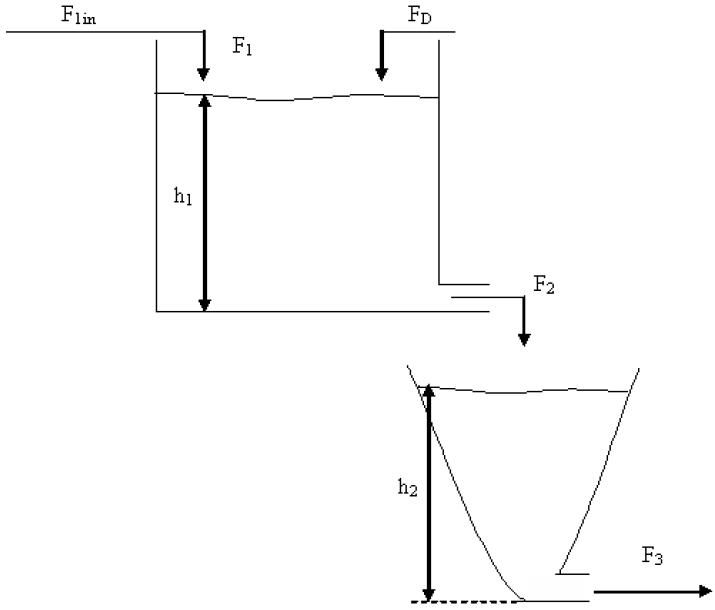
\includegraphics[width=0.8\textwidth]{pictures/schemat}
\caption{Obiekt regulacji automatycznej.}
\label{schemat}
\end{figure}

Wartością sterującą był dopływ $F_{1in}$ natomiast zakłóceniem - $F_D$. Z kolei wyjściem - wartością regulowaną - wysokość cieczy w drugim zbiorniku $h_2$. W pierwszej kolejności dokonano identyfikacji modelu, sprawdzono jego nieliniowość i dobrano odpowiedni rząd dynamiki modelu liniowego.
\chapter{Identyfikacja}
\section{Charakterystyka statyczna}
Poświęcono jej bardzo dużo uwagi, ze względu na kluczową rolę, jaką odgrywa we wspomnianych modelach Hammersteina i Wienera. Korzystając z modelu fizycznego, z równania \ref{model_fiz} wyznaczono:
\begin{equation}
\frac{dV_1}{dt} = 0 \quad \wedge \quad \frac{dV_2}{dt} = 0
\end{equation}

\noindent wobec tego:
\begin{equation}
\begin{cases}
F_1 + F_D - \alpha_1 \sqrt{h_1} &= 0 \\
\alpha_1 \sqrt{h_1} - \alpha_2 \sqrt{h_2} &= 0
\end{cases}
\end{equation}

\noindent Po prostych przekształceniach otrzymano wzór opisujący charakterystykę statyczną:
\begin{equation}
h_2 = \left( \frac{F_1 + F_D}{\alpha_2} \right)^2
\end{equation}

\noindent Wykres odpowiadający wyprowadzonemu wzorowi prezentuje się następująco:

\begin{figure}[h!]
\centering
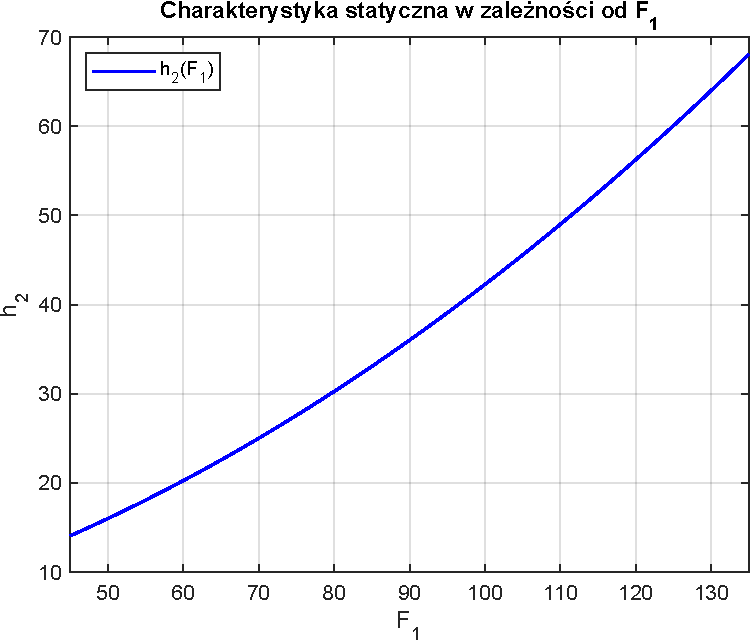
\includegraphics[width=0.8\textwidth]{pictures/static_characteristic}
\caption{Charakterystyka statyczna $h_2(F_1)$.}
\label{static_characteristic}
\end{figure}

\noindent Założono przedział zmienności sygnału sterującego w zakresie $F_1 \in [-45, 45]$.

\newpage

\section{Wymuszenia}
Po dokonaniu pierwszego kroku identyfikacji - wykreślenia charakterystyki statycznej - uzyskano wstępne informacje o obiekcie. Równania opisujące model (\ref{model_fiz}) oraz charakterystyka statyczna przedstawiona na rys. \ref{static_characteristic} pokazuje, że obiekt jest nieliniowy, stąd dokonano jego linearyzacji w punkcie pracy, tj.:
\begin{equation}
\begin{cases}
\frac{dV_1}{dt} \cong F_1 + F_D - \alpha_1 \sqrt{\frac{V_{10}}{A}} - \frac{\alpha_1}{2 \sqrt{A \cdot V_{10}}} \cdot (V_1 - V_{10})\\
\frac{dV_2}{dt} \cong \alpha_1 \sqrt{\frac{V_{10}}{A}} - \alpha_2 \sqrt[4]{\frac{V_{20}}{C}} + \frac{\alpha_1}{2 \sqrt{A \cdot V_{10}}} \cdot (V_1 - V_{10}) - \frac{\alpha_2}{4 \sqrt[4]{C \cdot V_{20}^3}} \cdot (V_2 - V_{20})
\end{cases}
\end{equation}

\noindent Linearyzacji dokonano przyjmując jako zmienną stanu objętość cieczy w obu zbiornikach. 

\begin{equation}
x = \begin{bmatrix} V_1 & V_2 \end{bmatrix}^T
\end{equation}

Następnie, podając wygenerowaną sekwencję sygnału sterującego, zbadano rozbieżność modelu liniowego i nieliniowego.

\begin{figure}[h!]
\centering
\subfloat[Wygenerowana sekwencja sygnału sterującego $u(k)$.]{
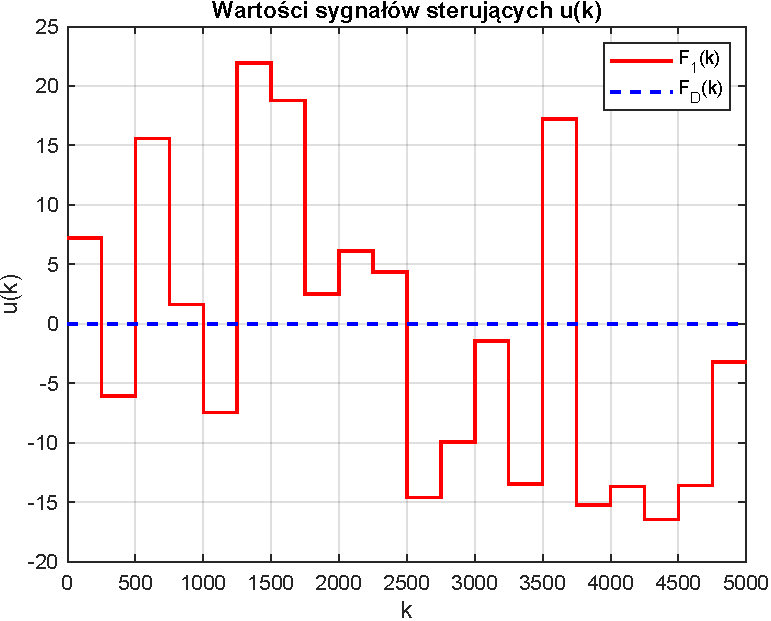
\includegraphics[width=0.45\textwidth]{pictures/u_F1}}
\hfill
\subfloat[Sygnał wyjściowy $y(k)$.]{
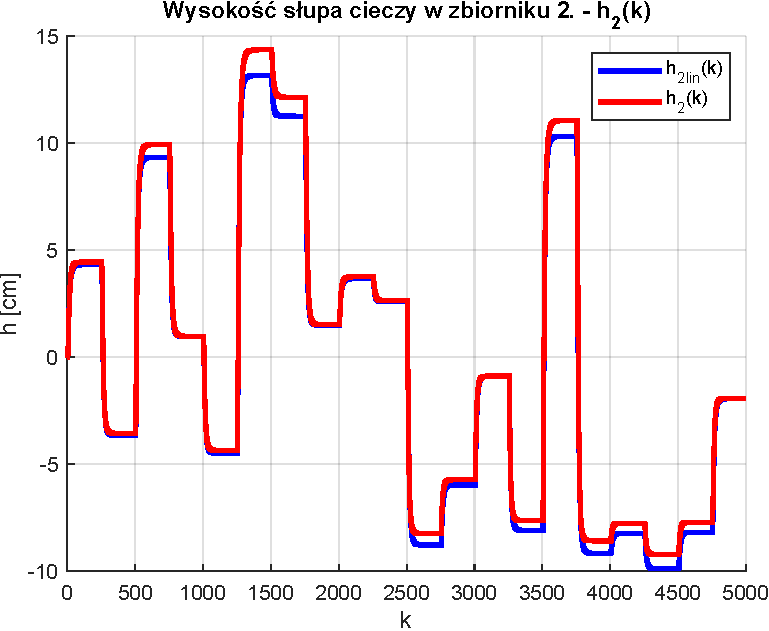
\includegraphics[width=0.45\textwidth]{pictures/y_F1}}
\caption{Porównanie modelu liniowego z nieliniowym.}
\end{figure}

Otrzymano dokładnie to czego się spodziewano. Wymuszenia nie większe niż $\pm 10 \frac{cm^3}{s}$ nie powodują znacznego wytrącenia układu z położenia równowagi, dzięki czemu model liniowy bardzo dobrze aproksymuje zachowanie układu. Niestety sytuacja pogarsza się wraz z oddalaniem się od punktu pracy - model liniowy zaczyna poważnie odbiegać od modelu nieliniowego, opisującego obiekt. W celach porównawczych policzono błędy, testując model w trybie bez rekurencji (ARX) oraz z rekurencją OE, przyjmując jako kryterium jakości błąd średni kwadratowy, tj.:

\begin{equation}
E = \sum_{k=0}^N (y(k) - y^{mod}(k))^2
\end{equation}

\noindent Wcześniej dokonano podziału wygenerowanych danych dynamicznych na dwa zbiory - uczący i~weryfikujący - stosując zasadę podziału $0\% - 50\% / 50\% - 100\%$, potrzebne do późniejszego, ewentualnego dostrajania modelu. Otrzymano następujące wyniki:

\begin{description}
\item[ARX] 
\begin{equation}
E_{ucz} = \num{0.002} \hspace{1cm} E_{wer}=\num{0.003}
\end{equation}
\item[OE] 
\begin{equation}
E_{ucz} = \num{0.470} \hspace{1cm} E_{wer}=\num{0.831}
\end{equation}
\end{description}

%\newpage

\begin{figure}[p!]
\begin{center}
\Large \textbf{Model ARX}
\end{center} 
\centering
\subfloat[Zbiór uczący.]{
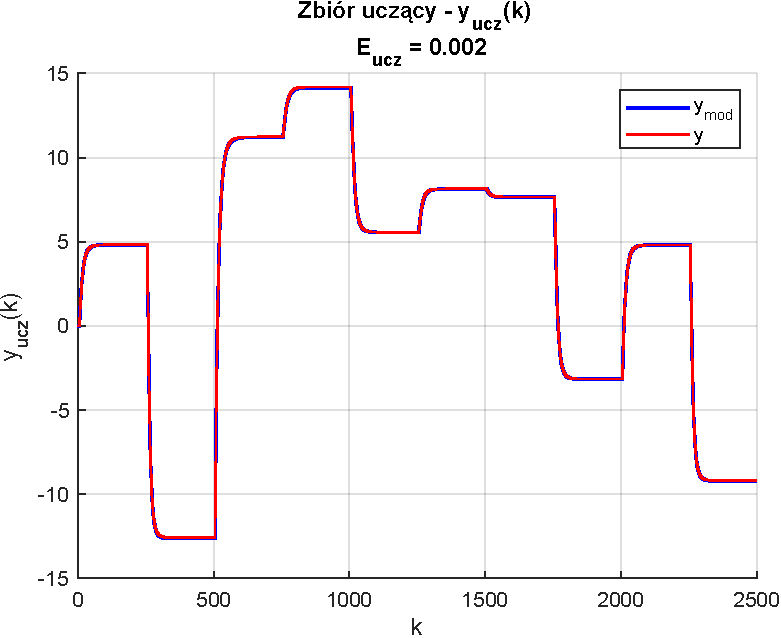
\includegraphics[width=0.45\textwidth]{pictures/arx_ucz}}
\hfill
\subfloat[Zbiór weryfikujący.]{
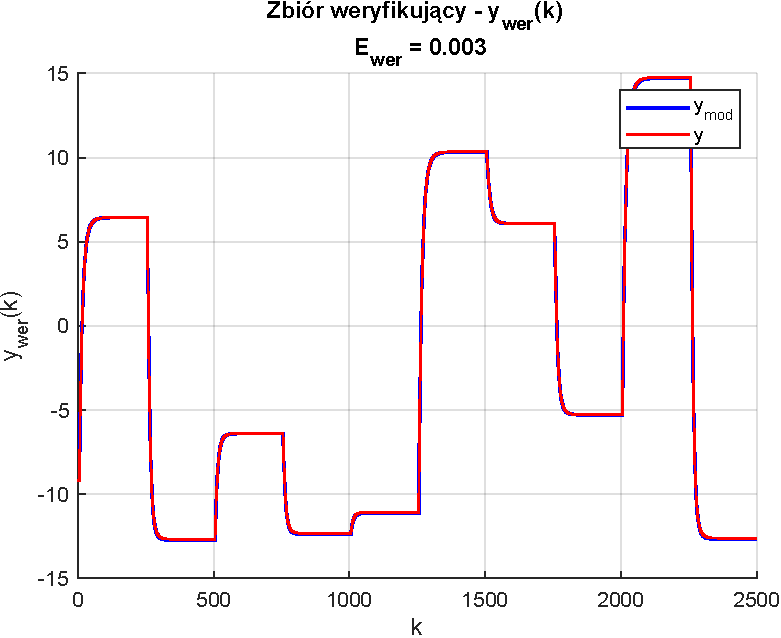
\includegraphics[width=0.45\textwidth]{pictures/arx_wer}}

\begin{center}
\Large \textbf{Model OE}
\end{center} 
\subfloat[Zbiór uczący.]{
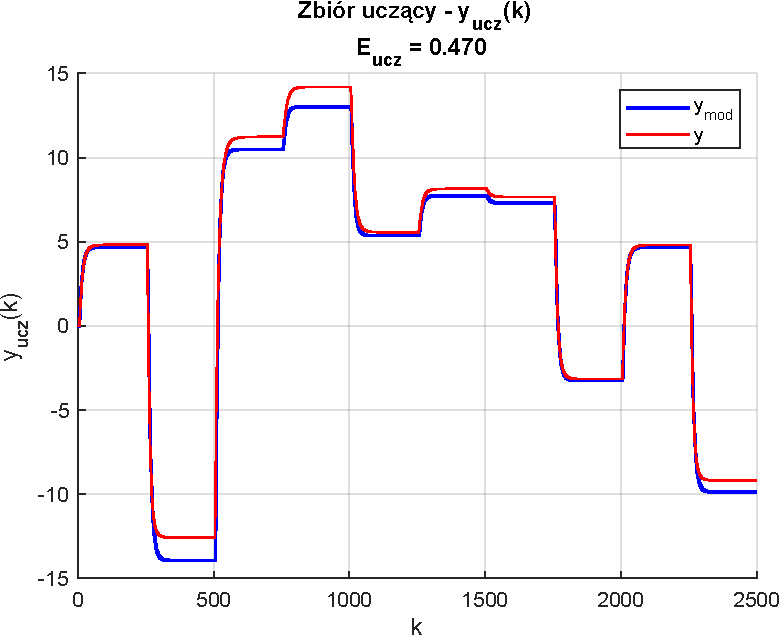
\includegraphics[width=0.45\textwidth]{pictures/oe_ucz}}
\hfill
\subfloat[Zbiór weryfikujący.]{
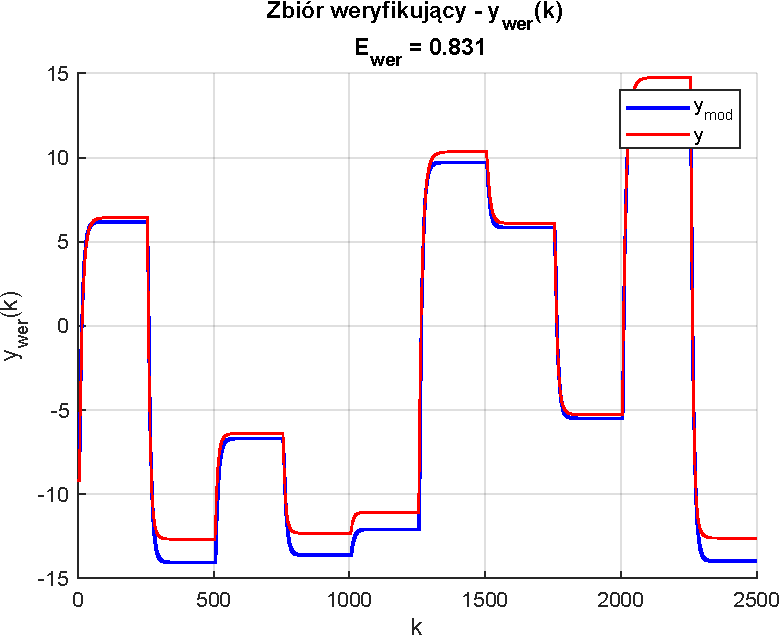
\includegraphics[width=0.45\textwidth]{pictures/oe_wer}}
\caption{Symulacja odpowiednich modeli z wykorzystaniem wygenerowanej sekwencji sygnału sterującego.}
\end{figure}

\newpage

\section{Podejście inżynierskie}
Od tej pory do dalszej analizy postanowiono przyjąć model szarej skrzynki. Informacją o obiekcie był fakt, że układ był inercyjny. Zadano więc wymuszenie w postaci skoku jednostkowego i starano się aproksymować odpowiedź układu dobierając odpowiednie parametru dla modelu transmitancji \textit{First Order Plus Dead Time} (FOPDT), który wyraża się wzorem:

\begin{equation}
G(s) = \frac{K_0e^{-sT_0}}{T_1s + 1}
\end{equation}

\noindent Dobrane parametry:

\begin{equation}
K_0 = \num{0.6025} \hspace{1cm} T_0 = 100 \hspace{1cm} T_1 = 225
\end{equation}

\begin{figure}[h!]
\centering
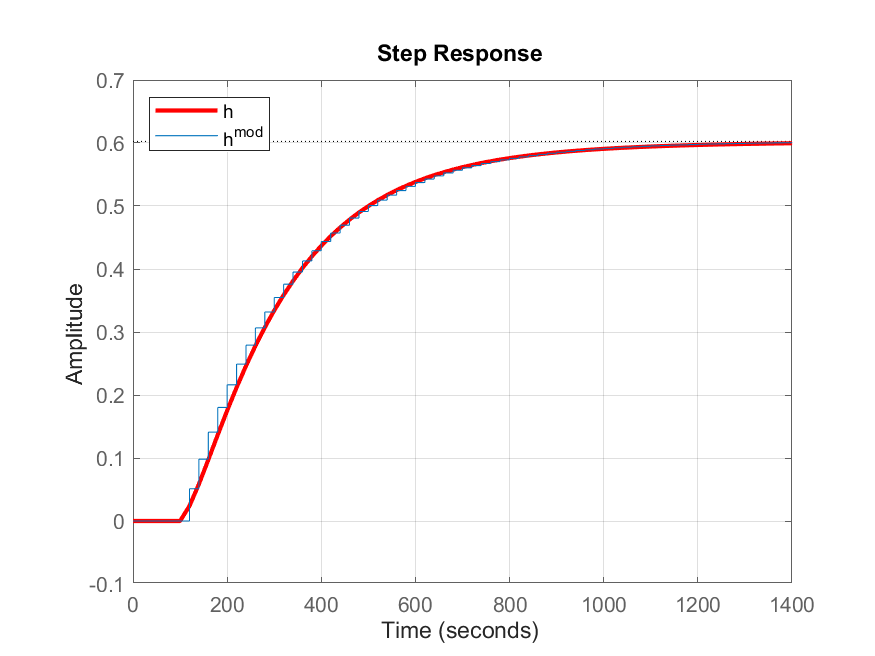
\includegraphics[width=\textwidth]{pictures/model_fopdt}
\caption{Aproksymacja odpowiedzi skokowej układu modelem FOPDT.}
\end{figure}

\newpage

Uzyskany rezultat nie był satysfakcjonujący stąd przyjęto model \textit{Second Order Plus Dead Time} (SOPDT), tj.

\begin{equation}
G(s) = \frac{K_0e^{-sT_0}}{(T_1s + 1)(T_2s + 1)}
\end{equation}

\noindent Dobrane parametry:

\begin{equation}
K_0 = \num{0.6025} \hspace{1cm} T_0 = 100 \hspace{1cm} T_1 = 212 \hspace{1cm} T_2 = 15
\end{equation}

\noindent Wynik prezentował się następująco:

\begin{figure}[h!]
\centering
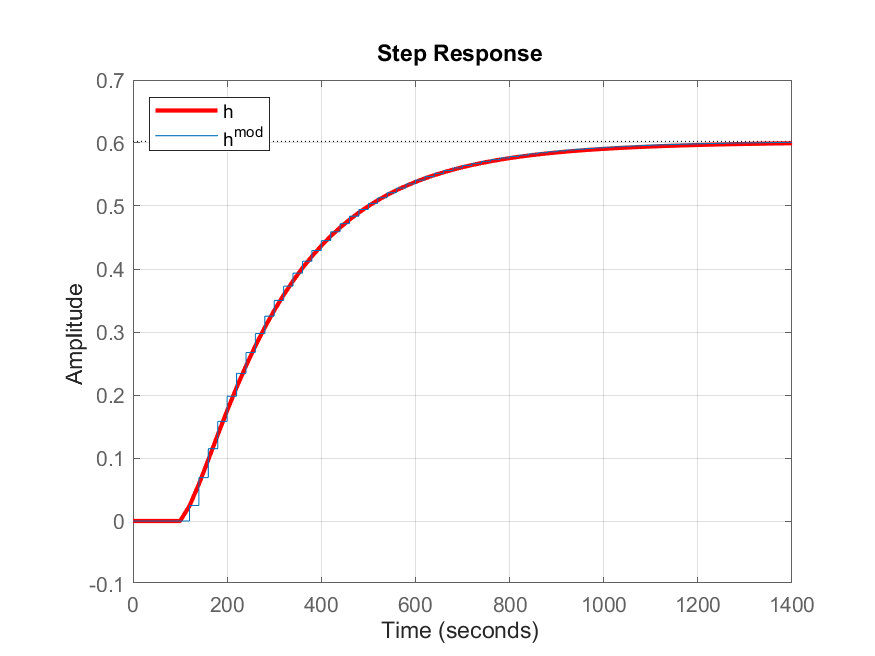
\includegraphics[width=\textwidth]{pictures/model_sopdt}
\caption{Aproksymacja odpowiedzi skokowej układu modelem SOPDT.}
\end{figure}

\newpage

Ponownie, chcąc sprawdzić skuteczność aproksymacji obiektu regulacji wygenerowanym modelem, którego równanie różnicowe jest postaci:

\begin{equation}
\begin{aligned}
y(k) = \num{1.174} y(k-1) - \num{0.2399} y(k-2) + &\num{0.02459} u_1(k-6) + \num{0.01536} u_1(k-7) \\ 
+&\num{0.02459} u_2(k-1) + \num{0.01536} u_2(k-2) 
\end{aligned}
\label{diff_eq}
\end{equation}

\noindent wygenerowano sekwencję sygnału sterującego $u_1(k)$ oraz $u_2(k)$, który są przyrostami wartości sterujących odpowiednio $F_1$ oraz $F_D$.

\begin{figure}[h!]
\begin{center}
\Large \textbf{Model ARX}
\end{center} 
\centering
\subfloat[Zbiór uczący.]{
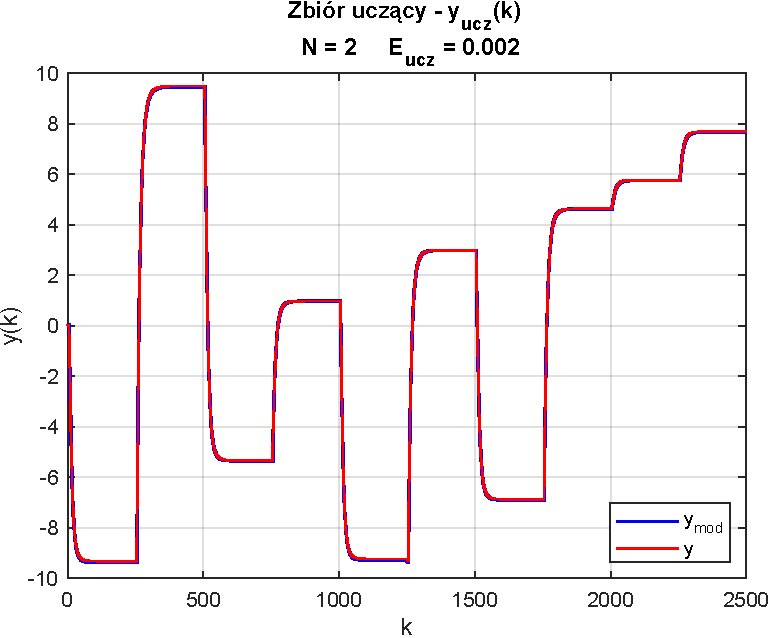
\includegraphics[width=0.45\textwidth]{pictures/arx_ucz_sopdt}}
\hfill
\subfloat[Zbiór weryfikujący.]{
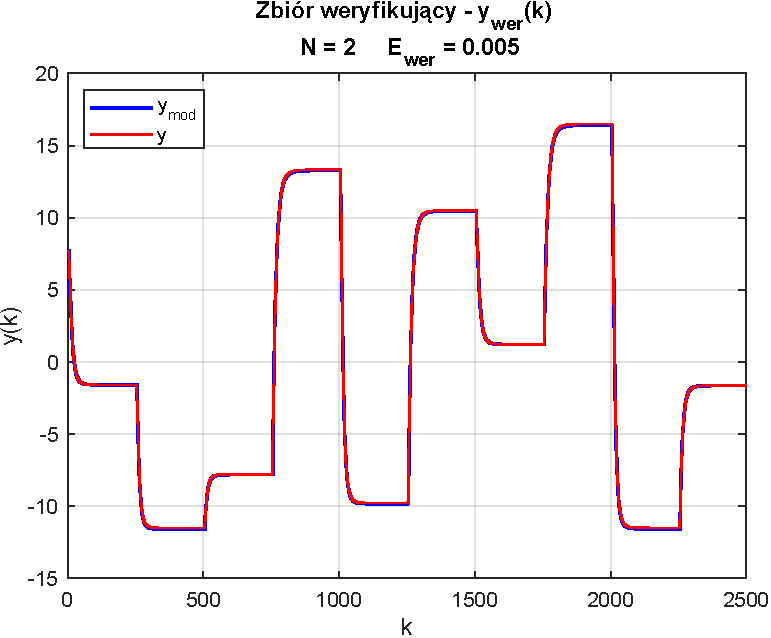
\includegraphics[width=0.45\textwidth]{pictures/arx_wer_sopdt}}

\begin{center}
\Large \textbf{Model OE}
\end{center} 
\subfloat[Zbiór uczący.]{
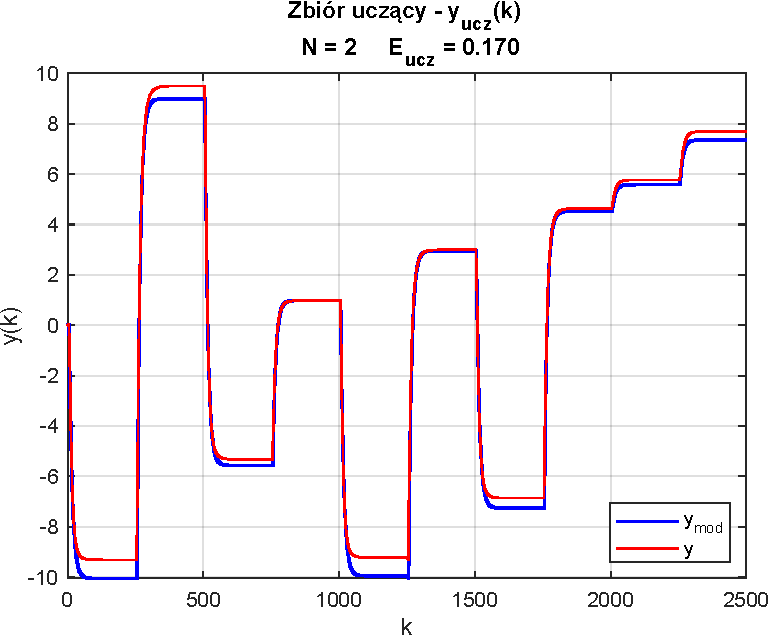
\includegraphics[width=0.45\textwidth]{pictures/oe_ucz_sopdt}}
\hfill
\subfloat[Zbiór weryfikujący.]{
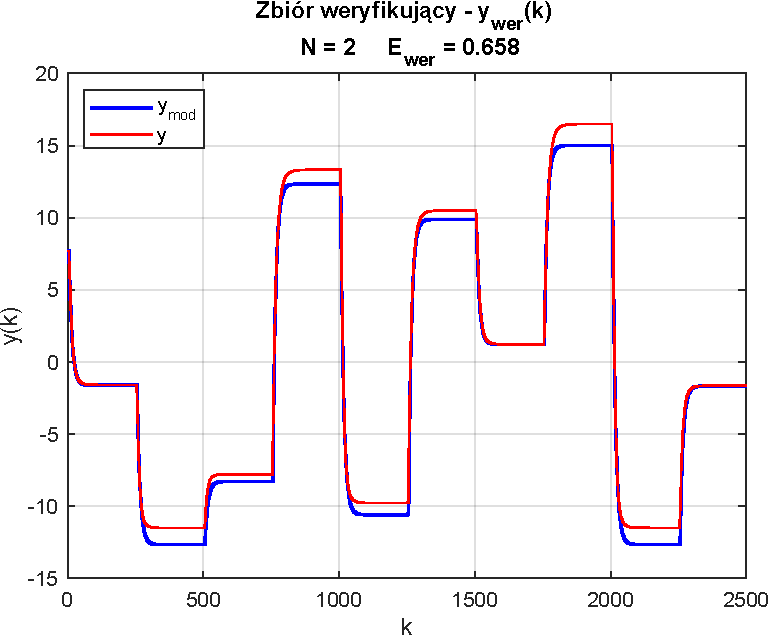
\includegraphics[width=0.45\textwidth]{pictures/oe_wer_sopdt}}
\caption{Symulacja odpowiednich modeli z wykorzystaniem wygenerowanej sekwencji sygnału sterującego.}
\end{figure}

Błędy uznano za akceptowalne na tym poziomie identyfikacji i przyjęto wyznaczony model do dalszej analizy.
\section{Model Hammersteina}
Po przeanalizowaniu charakterystyki statycznej oraz porównaniu modelu nieliniowego z liniowym przystąpiono do identyfikacji modelu Hammersteina.
Istota polega na umieszczeniu nieliniowego bloku statycznego przed liniowym blokiem dynamicznym, co pozwala na oddzielenie nieliniowości od dynamiki systemu. Jego główną zaletą jest prostsza identyfikacja parametrów, ponieważ najpierw określa się charakterystykę statyczną, a dopiero potem analizuje dynamikę. Takie podejście lepiej odwzorowuje systemy, w których nieliniowości wynikają z właściwości aktuatorów lub czujników, a część dynamiczna pozostaje liniowa. Graficzne ujęcie opisanego modelu zilustrowano na rys. \ref{hamm_model}.

\begin{figure}[h!]
\centering
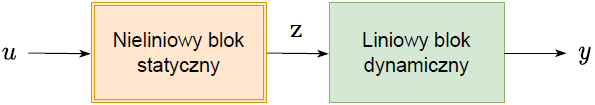
\includegraphics[width=\textwidth]{pictures/hamm_model}
\caption{Reprezentacja graficzna modelu Hammersteina.}
\label{hamm_model}
\end{figure}

\noindent Cała procedura w przypadku analizowanego obiektu wygląda następująco, sygnał sterujący jest wejściem nieliniowego bloku statycznego, którego wyjściem jest przekonwertowany sygnał $z = f(u)$. Następnie sygnał $z$ trafia do liniowego bloku dynamicznego. Dzięki temu rozdzieleniu nieliniowości i dynamiki, możliwe jest zastosowanie klasycznych metod projektowania regulatorów dla części dynamicznej, co upraszcza proces sterowania.

\subsection{Nieliniowy blok statyczny}
Nieliniowość w charakterystyce statycznej została wprowadzono za pomocą logiki rozmytej (ang. \textit{fuzzy logic}), a konkretnie za pomocą modeli rozmytych Takagi-Sugeno. Zastosowano dwa podejścia, jedno standardowe z następnikami liniowymi, natomiast drugie z następnikami hiperbolicznymi.

\subsection{Następniki liniowe}
W standardowej wersji modeli Takagi-Sugeno następniki przyjmują liniową postać, dlatego to właśnie od nich postanowiono zacząć. Rozmyto zmienną wejściową oraz wybrano odpowiednią liczbę zbiorów rozmytych. Zastosowano następniki liniowe postaci:

\begin{equation}
\begin{aligned}
\text{Reguła 1: Jeśli} \quad u(k) \quad \text{jest} \quad &U_1, \quad \text{to}: \quad y^1(k) = a_1 u(k) + b_1 \\[10pt]
\text{Reguła 2: Jeśli} \quad u(k) \quad \text{jest} \quad &U_2, \quad \text{to}: \quad y^2(k) = a_2 u(k) + b_2 \\[10pt]
&\vdots \\[10pt]
\text{Reguła 5: Jeśli} \quad u(k) \quad \text{jest} \quad &U_5, \quad \text{to}: \quad y^2(k) = a_5 u(k) + b_5 \\[10pt]
\end{aligned}
\label{nastepniki_lin}
\end{equation}

\noindent Natomiast wyjście systemu rozmytego obliczano zgodnie ze wzorem \ref{wniosek}.

\newpage

\begin{figure}[h!]
\centering
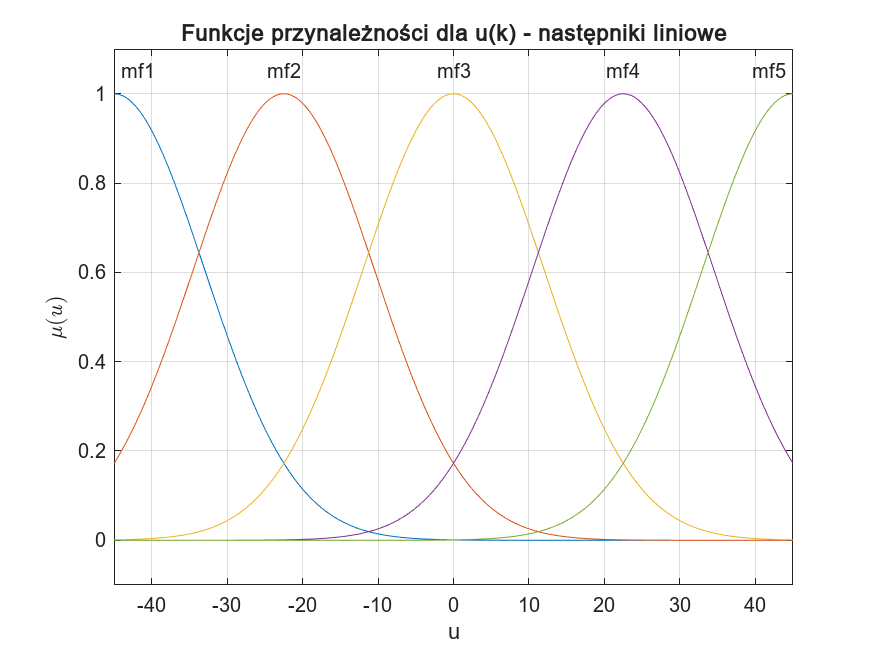
\includegraphics[width=\textwidth]{pictures/hamm_linearFis}
\caption{Zbiory rozmyte - następniki liniowe.}
\end{figure}

Zarówno do budowy modelu, jak i wyznaczenia parametrów następników wykorzystano narzędzia oferowane przez MATLAB w ramach \textit{Fuzzy Logic Toolbox}. Korzystając z funkcji \verb+sugfis()+ zbudowano nieliniowy model rozmyty typu Takagi - Sugeno. Zdecydowano się na pięć zbiorów rozmytych o gaussowskim kształcie, co zapewnia różniczkowalność (SZAU). Następnie, dzięki wykorzystaniu \verb+addInput()+, \verb+addOutput()+, \verb+addMF()+ udało się zbudować bazę reguł - \verb+addRule()+, co bezpośrednio przełożyło się na wyznaczenie współczynników pierwszej iteracji. Konieczne było późniejsze ręczne dostrajanie modelu, które przy względnie dużej liczbie zbiorów nie przysporzyło dużo problemów. Ostatecznie zdefiniowano następujące wartości parametrów następników:

\begin{table}[h!]
\centering
\renewcommand{\arraystretch}{1.2} % Zwiększa wysokość wierszy
\begin{tabular}{|>{\centering\arraybackslash}m{3cm}|>{\centering\arraybackslash}m{3cm}|>{\centering\arraybackslash}m{3cm}|}
\hline
Nr reguły & Współczynnik $a_r$ & Współczynnik $b_r$ \\ \hline
1 & $\num{0.7895}$ & $\num{0.0001}$ \\ \hline
2 & $\num{0.8982}$ & $\num{0.0002}$ \\ \hline
3 & $\num{1.0933}$ & $\num{0.0001}$ \\ \hline
4 & $\num{1.0489}$ & $\num{0}$ \\ \hline
5 & $\num{1.2034}$ & $\num{0.0001}$ \\ \hline
\end{tabular}
\end{table}

\newpage

\subsection{Następniki nieliniowe}
Wprowadzając następniki w postaci hiperbolicznej spodziewano się zachowania dokładności przy jednoczesnym zmniejszeniu liczby zbiorów rozmytych [Robust observer-based controller design for Takagi–Sugeno systems with nonlinear consequent parts]. Sformułowano następującą bazę reguł:

\begin{equation}
\begin{aligned}
\text{Reguła 1: Jeśli} \quad u(k) \quad \text{jest} \quad &U_1, \quad \text{to}: \quad y^1(k) = a_1 \sinh\left(\frac{u(k)}{b_1}\right) \\[10pt]
\text{Reguła 2: Jeśli} \quad u(k) \quad \text{jest} \quad &U_2, \quad \text{to}: \quad y^2(k) = a_2 \sinh\left(\frac{u(k)}{b_2}\right) \\[10pt]
\text{Reguła 3: Jeśli} \quad u(k) \quad \text{jest} \quad &U_3, \quad \text{to}: \quad y^2(k) = a_3 \sinh\left(\frac{u(k)}{b_3}\right)
\end{aligned}
\label{nastepniki_nlin}
\end{equation}

Zgodnie z oczekiwaniami udało się wprowadzić mniejszą liczbę zbiorów rozmytych.

\begin{figure}[h!]
\centering
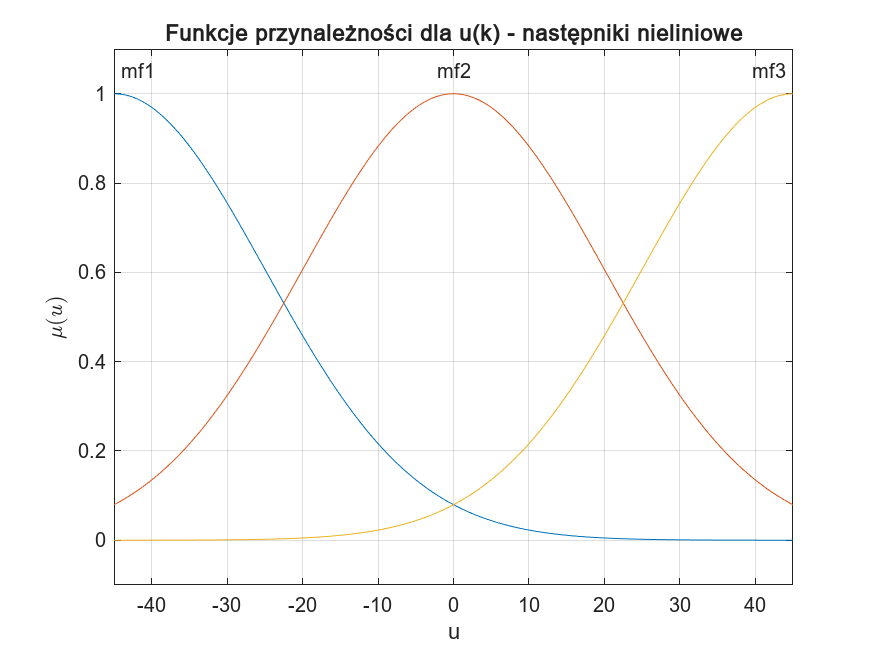
\includegraphics[width=\textwidth]{pictures/hamm_nonlinearFis}
\caption{Zbiory rozmyte - następniki nieliniowe.}
\end{figure}

\newpage

Procedura dostrajania parametrów następników różniła się w stosunku do odpowiedników liniowych. Wynikało to z tego, że wykorzystywane narzędzie do budowy modelu rozmytego domyślnie stroi parametry dla następników liniowych, stąd konieczność znacznej modyfikacji i ręcznego dostrajania. Następnie, po ręcznym dostrojeniu wykorzytsano funkcję z pakietu \textit{Optimization Toolbox}, mianowicie \verb+fminsearch()+. Wybrano taką kolejność ze względu na fakt, że odwracając kolejność, tzn. stosując najpierw metodę Neldera-Meada, otrzymywane wyniki były gorsze niż te wybrane ręcznie. Było to spowodowane skłonnością do wpadania algorytmu w minima lokalne. Istotnym aspektem w tym przypadku okazała się normalizacja argumentu, bowiem kształt funkcji $\sinh()$ zmienia się bardzo gwałtownie dla rosnących wartości zmiennej (rys. {\ref{sinh}}. 

\begin{figure}[h!]
\centering
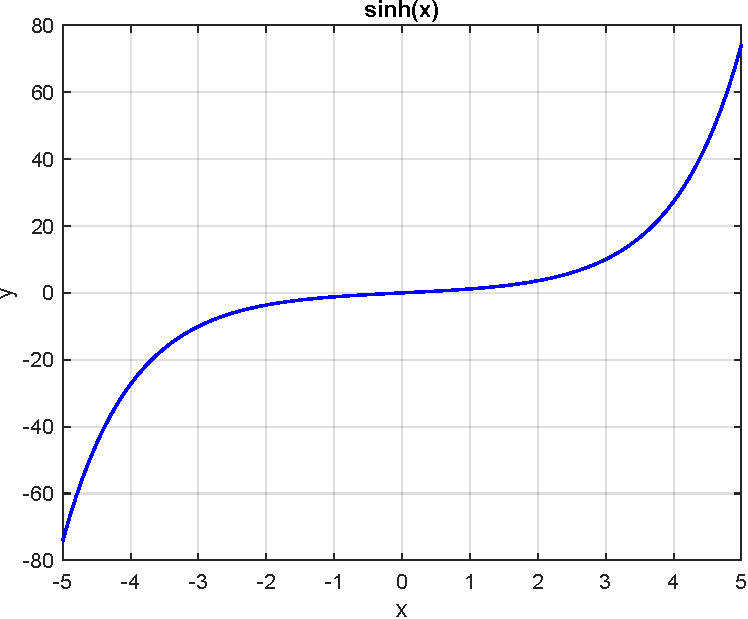
\includegraphics[width=\textwidth]{pictures/sinh}
\caption{Wykres funkcji $\sinh()$.}
\label{sinh}
\end{figure}

Ostateczne wartości współczynników następników reguł zebrano w tab. \ref{nonlinear_coeff}.

\begin{table}[h!]
\centering
\renewcommand{\arraystretch}{1.2} % Zwiększa wysokość wierszy
\begin{tabular}{|>{\centering\arraybackslash}m{2cm}|>{\centering\arraybackslash}m{3cm}|>{\centering\arraybackslash}m{3cm}|}
\hline
Nr reguły & Współczynnik $a_r$ & Współczynnik $b_r$ \\ \hline
1. & $\num{46.4941}$ & $\num{62.8862}$ \\ \hline
2. & $\num{36.2347}$ & $\num{36.2592}$ \\ \hline
3. & $\num{110.4841}$ & $\num{98.7690}$ \\ \hline    
\end{tabular}
\caption{Współczynniki hiperbolicznych następników reguł.}
\label{nonlinear_coeff}
\end{table}

\newpage

\subsection{Porównanie}
Dostroiwszy oba modele przyszedł czas na ich porównanie. Wygenerowano pięć sekwencji losowo zmieniającego się sygnału sterującego, następnie wynik został porównany do rezultatu uzyskanego dla modelu nieliniowego - wzorcowego - obliczonego za pomocą zmodyfikowanej metody Eulera. Wskaźnikiem porównawczym był błąd średnio kwadratowy. Aby zaznaczyć jakie korzyści wnosi nieliniowa część modelu Hammersteina na dokładność modelowania, w każdej sekwencji obliczono także wskaźnik dla modelu liniowego.

\begin{figure}[h!]
\centering
\subfloat[Następniki liniowe]{
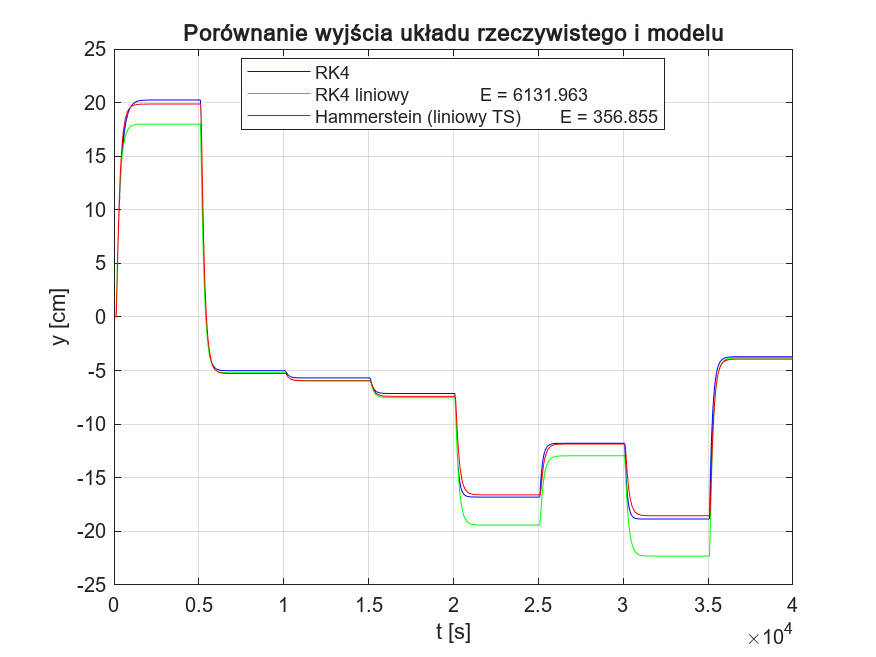
\includegraphics[width=0.7\textwidth]{pictures/HammersteinLinearModel_1}}
\vspace{0.5cm}
\subfloat[Następniki nieliniowe]{
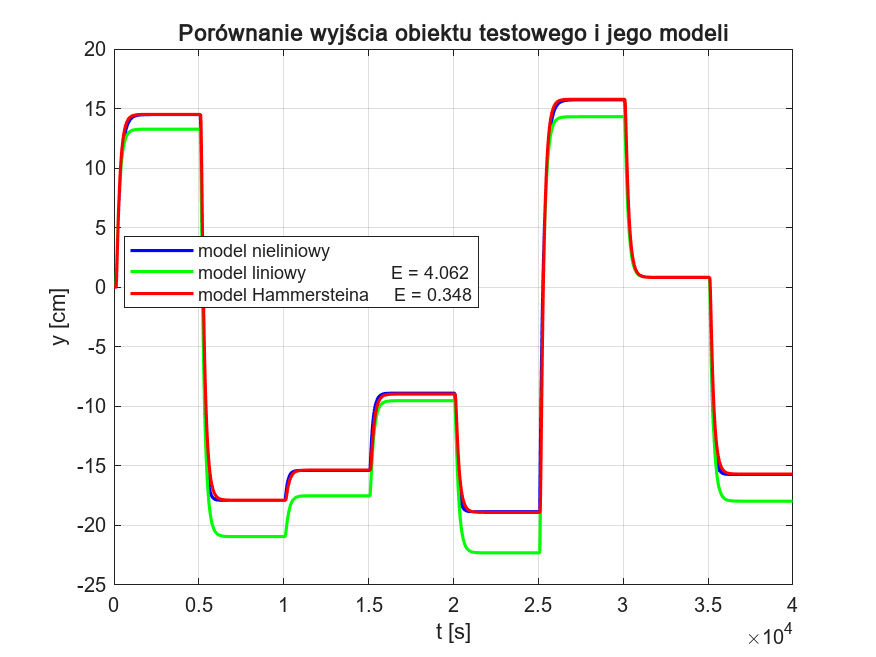
\includegraphics[width=0.7\textwidth]{pictures/HammersteinNonlinearModel_1}}
\caption{Porównanie modelu Hammersteina z następnikami liniowymi i nieliniowymi - pierwsza sekwencja.}
\label{first_hamm}
\end{figure}

\begin{figure}[p]
\centering
\subfloat[Następniki liniowe]{
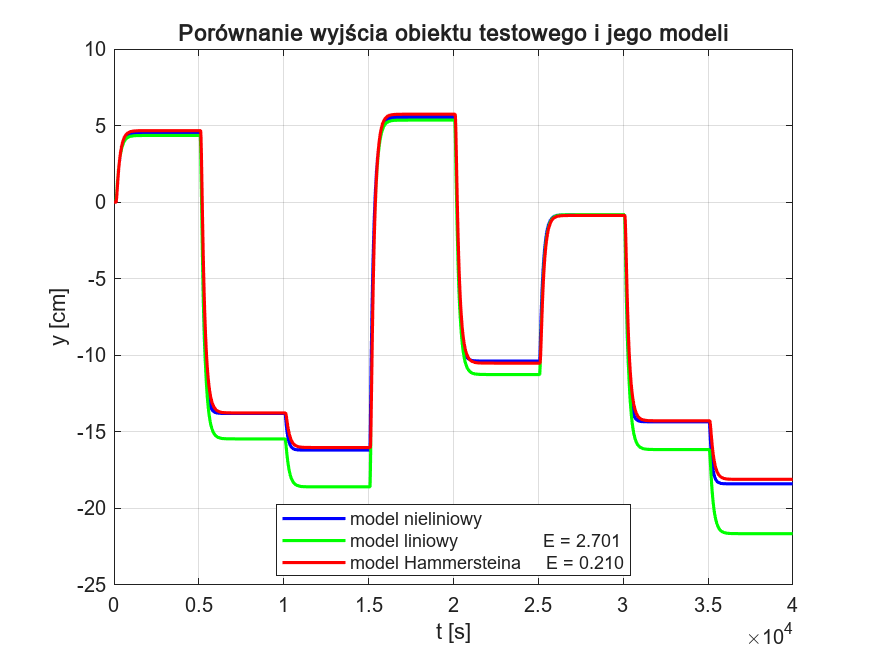
\includegraphics[width=0.75\textwidth]{pictures/HammersteinLinearModel_2}}
\vspace{0.5cm}
\subfloat[Następniki nieliniowe]{
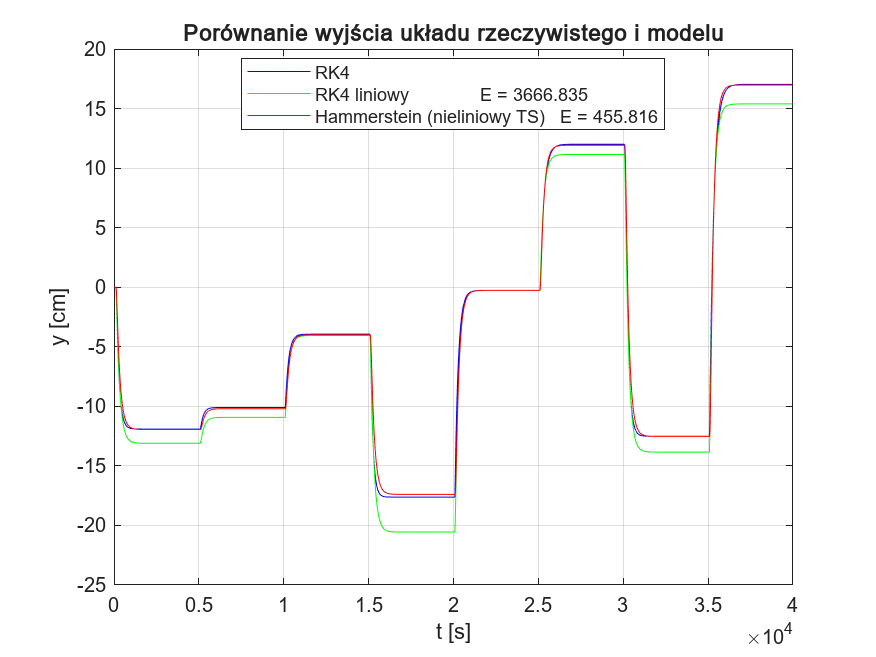
\includegraphics[width=0.75\textwidth]{pictures/HammersteinNonlinearModel_2}}
\caption{Porównanie modelu Hammersteina z następnikami liniowymi i nieliniowymi - druga sekwencja.}
\end{figure}

\begin{figure}[p]
\centering
\subfloat[Następniki liniowe]{
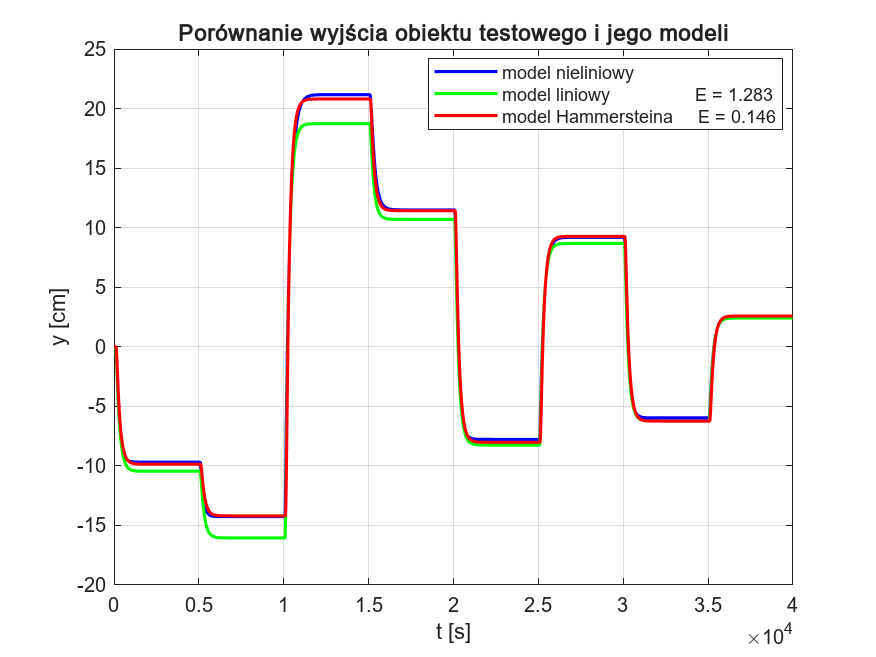
\includegraphics[width=0.75\textwidth]{pictures/HammersteinLinearModel_3}}
\vspace{0.5cm}
\subfloat[Następniki nieliniowe]{
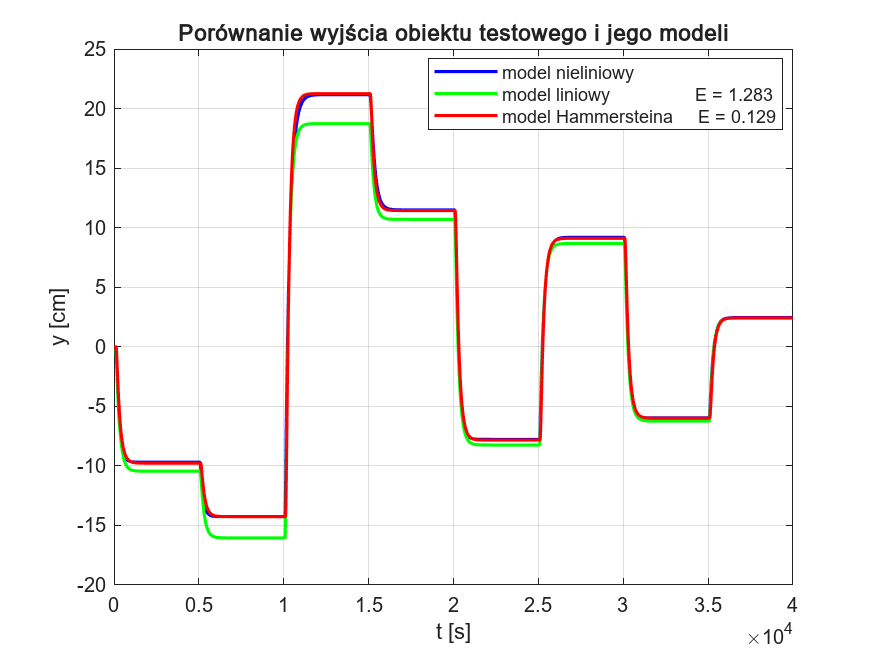
\includegraphics[width=0.75\textwidth]{pictures/HammersteinNonlinearModel_3}}
\caption{Porównanie modelu Hammersteina z następnikami liniowymi i nieliniowymi - trzecia sekwencja.}
\end{figure}

\begin{figure}[p]
\centering
\subfloat[Następniki liniowe]{
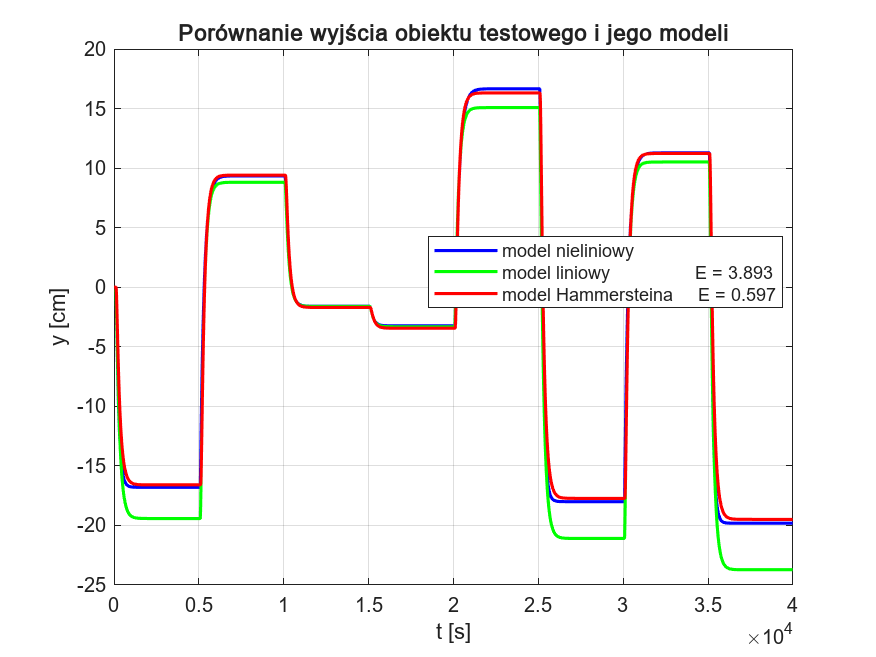
\includegraphics[width=0.75\textwidth]{pictures/HammersteinLinearModel_4}}
\vspace{0.5cm}
\subfloat[Następniki nieliniowe]{
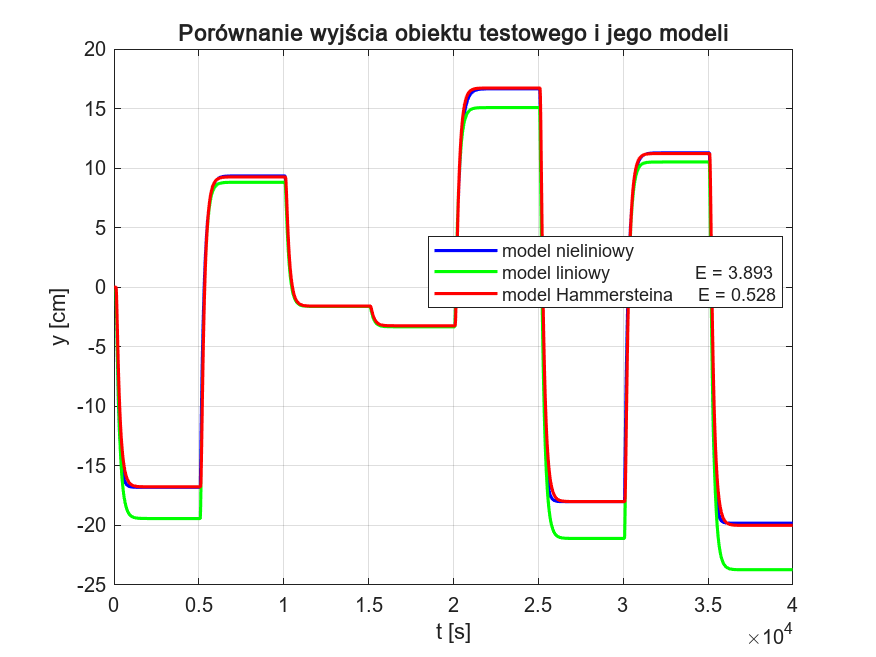
\includegraphics[width=0.75\textwidth]{pictures/HammersteinNonlinearModel_4}}
\caption{Porównanie modelu Hammersteina z następnikami liniowymi i nieliniowymi - czwarta sekwencja.}
\end{figure}

\begin{figure}[p]
\centering
\subfloat[Następniki liniowe]{
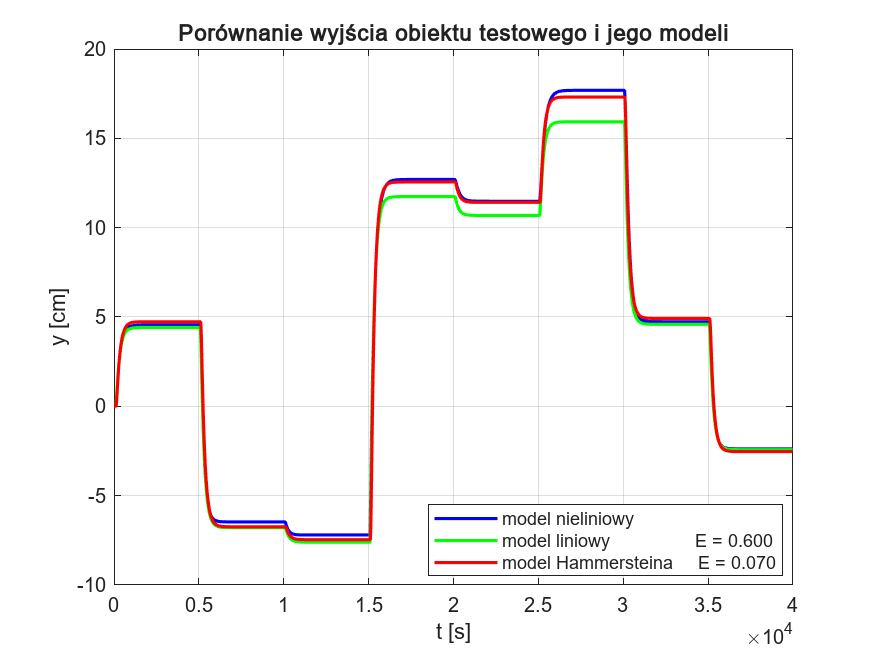
\includegraphics[width=0.75\textwidth]{pictures/HammersteinLinearModel_5}}
\vspace{0.5cm}
\subfloat[Następniki nieliniowe]{
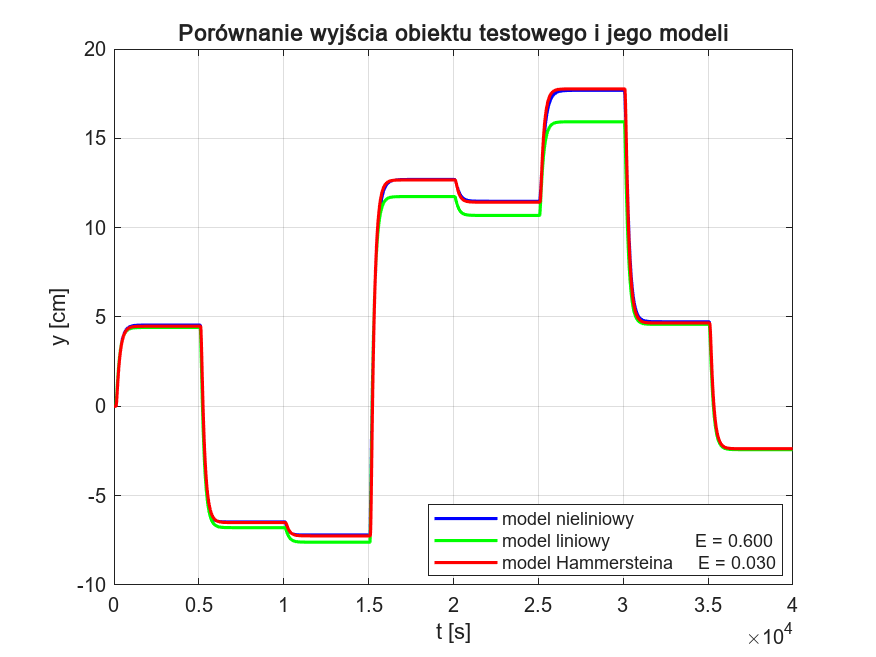
\includegraphics[width=0.75\textwidth]{pictures/HammersteinNonlinearModel_5}}
\caption{Porównanie modelu Hammersteina z następnikami liniowymi i nieliniowymi - piąta sekwencja.}
\label{last_hamm}
\end{figure}

\newpage

Zaprezentowane wykresy na rys. \ref{first_hamm} - \ref{last_hamm} ilustrują przede wszystkim zysk zastosowania modelu Hammersteina do opisu obiektu. Otrzymane wyniki są nieporównywalnie lepsze w stosunku do modelu liniowego. Natomiast przyglądając się z bliska, można zauważyć również poprawę dzięki wprowadzeniu dodatkowej nieliniowości w definicji następników rozmytego modelu typu Takagi-Sugeno. W tab. \ref{comparison_hamm} zebrano uzyskane wyniki.

\begin{table}[h!]
\centering
\renewcommand{\arraystretch}{1.2}
\begin{tabular}{|>{\centering\arraybackslash}m{2cm}|>{\centering\arraybackslash}m{3cm}|>{\centering\arraybackslash}m{3cm}|>{\centering\arraybackslash}m{3cm}|}
\hline
\multirow{2}{*}{Nr sekwencji} & \multirow{2}{*}{Model liniowy} & \multicolumn{2}{c|}{Model Hammersteina} \\ \cline{3-4}
 &  & Następniki liniowe & Następniki nieliniowe \\ \hline
1. & $\num{4.062}$ & $\num{0.395}$ & $\num{0.348}$ \\ \hline
2. & $\num{2.701}$ & $\num{0.210}$ & $\num{0.177}$ \\ \hline
3. & $\num{1.283}$ & $\num{0.146}$ & $\num{0.129}$ \\ \hline
4. & $\num{3.893}$ & $\num{0.597}$ & $\num{0.528}$ \\ \hline
5. & $\num{0.600}$ & $\num{0.070}$ & $\num{0.030}$ \\ \hline
\end{tabular}
\caption{Porównanie modeli.}
\label{comparison_hamm}
\end{table}

Należy pamiętać, że w przypadku następników hiperbolicznych zredukowano liczbę zbiorów rozmytych. Zatem udało się poprawić dokładność modelowania, przy jednoczesnym zmniejszeniu liczby reguł modelu TS.
\section{Model Wienera}
Model Wienera to struktura nieliniowego systemu, w której liniowy blok dynamiczny jest umieszczony przed nieliniowym blokiem statycznym. Oznacza to, że najpierw wejście przechodzi przez liniowy filtr, a następnie poddawane jest nieliniowej transformacji. Modele Wienera są szczególnie użyteczne w systemach, gdzie obserwowana nieliniowość wynika głównie z ograniczeń lub nasycenia elementów wykonawczych, takich jak silniki, zawory, czy inne elementy mechaniczne.  Zatem istota tego modeli jest taka sama jak w przypadku modelu Hammersteina - oddzielenie nieliniowej statyki od liniowej dynamiki - z tym, że nieliniową statykę poprzedzono liniową dynamika - odwrotnie niż jak to było w przypadku omówionego modelu, co graficznie zilustrowano na rys. \ref{wien_model}.

\begin{figure}[h!]
\centering
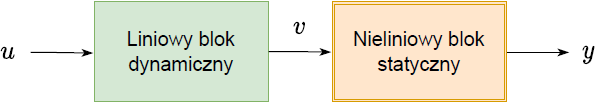
\includegraphics[width=\textwidth]{pictures/wien_model}
\caption{Reprezentacja graficzna modelu Wienera.}
\label{wien_model}
\end{figure}

Sygnał wejściowy trafia na liniowy blok dynamiczny, którego wyjściem jest przekonwertowany sygnał $v = f(u)$, który następnie trafia na nieliniową statykę, której wyjściem jest sygnał $y$.

Warto podkreślić, że modele Wienera jest trudniejszy w interpretacji niż model Hammersteina. Wynika to z tego, że sygnał wejściowy przechodzi najpierw przez system liniowy, a dopiero potem przez nieliniowy element, co utrudnia analizę wpływu nieliniowości. Dodatkowo, sygnał po filtracji liniowej może mieć bardziej złożone właściwości, co komplikuje ocenę jego zachowania w bloku nieliniowym, a także może przełożyć się na bardziej wymagającą estymacja parametrów w modelu.

\subsection{Następniki}
Zarówno w przypadku następników liniowych, jak i hiperbolicznych wykorzystano dokładnie te same definicje, jakie zastosowano w przypadku modelu Hammersteina - opisane wzorami \ref{nastepniki_lin} oraz \ref{nastepniki_nlin}. Przypomniano jedynie ogólną strukturę poszczególnych reguł.

\begin{description}
\item Następniki liniowe:
\begin{equation}
\text{Reguła n: Jeśli} \quad u(k) \quad \text{jest} \quad U_n, \quad \text{to}: \quad y^n(k) = a_n u(k) + b_n \\[10pt]
\end{equation}

\item Następniki hiperboliczne:
\begin{equation}
\text{Reguła n: Jeśli} \quad u(k) \quad \text{jest} \quad U_n, \quad \text{to}: \quad y^n(k) = a_n \sinh\left(\frac{u(k)}{b_n}\right) \\[10pt]
\end{equation}
\end{description}

\newpage

Nie uległa zmianie również liczba i postać zbiorów rozmytych - zmienił się jedynie zakres rozmywania. 

\begin{figure}[h!]
\centering
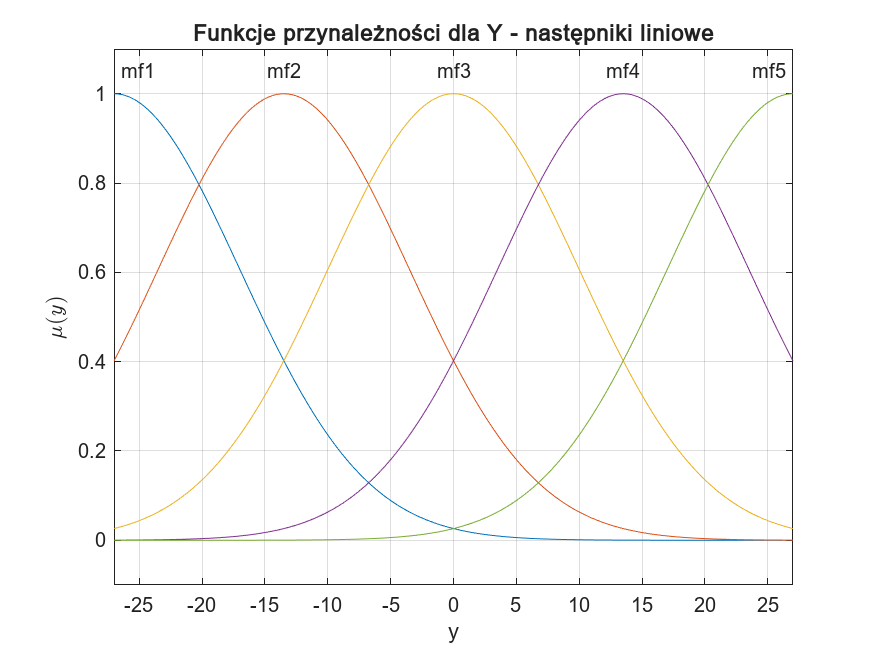
\includegraphics[width=0.85\textwidth]{pictures/WienerfuzzySets_liniowe}
\caption{Zbiory rozmyte - następniki liniowe.}
\end{figure}

\vfill

\begin{figure}[h!]
\centering
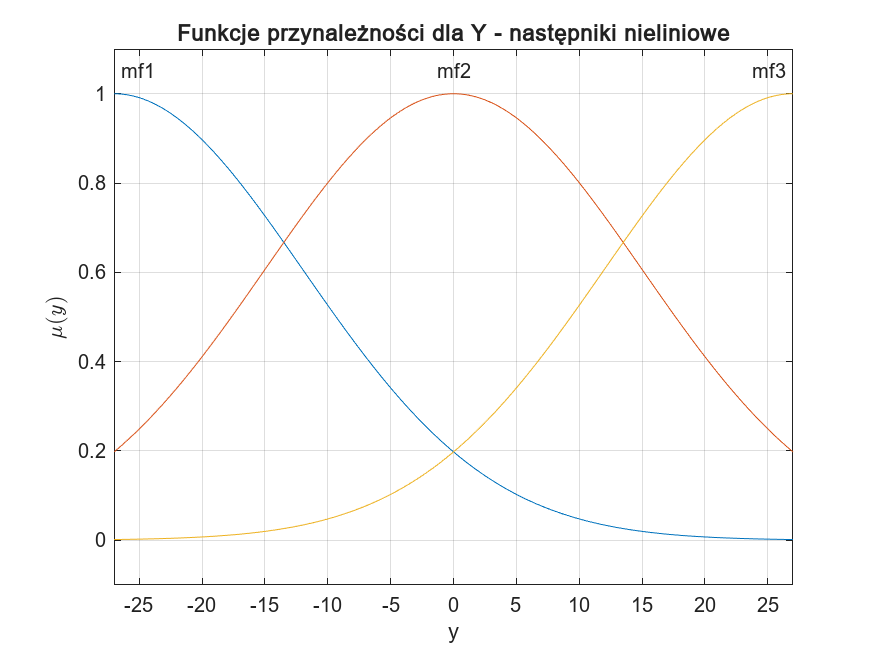
\includegraphics[width=0.85\textwidth]{pictures/WienerfuzzySets_nieliniowe}
\caption{Zbiory rozmyte - następniki nieliniowe.}
\end{figure}

\newpage

\subsection{Porównanie}

Procedura porównawcza wyglądała identycznie jak w przypadku modelu Hammersteina, tj. dla tych samych wygenerowanych sekwencji sygnału sterującego wyznaczono odpowiedzi modelu nieliniowego, liniowego, modelu Wienera z następnikami liniowymi oraz hiperbolicznymi. Przebiegi przedstawiono na rys. \ref{first_wien} - \ref{last_wien}, natomiast dane liczbowe zgromadzono w tab. \ref{comparison_wien}.

\begin{figure}[h!]
\centering
\subfloat[Następniki liniowe]{
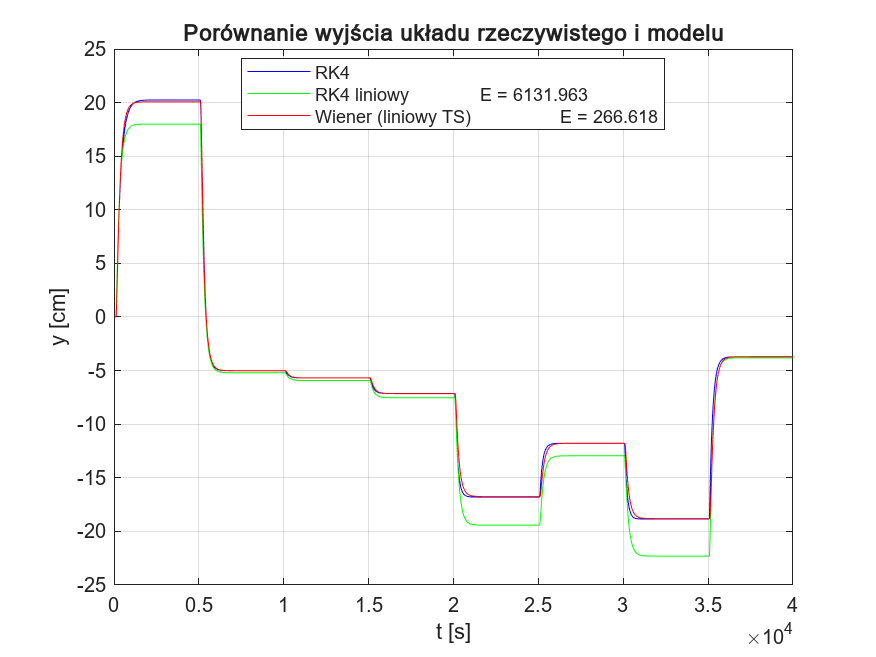
\includegraphics[width=0.7\textwidth]{pictures/WienerLinearModel_1}}
\vspace{0.5cm}
\subfloat[Następniki nieliniowe]{
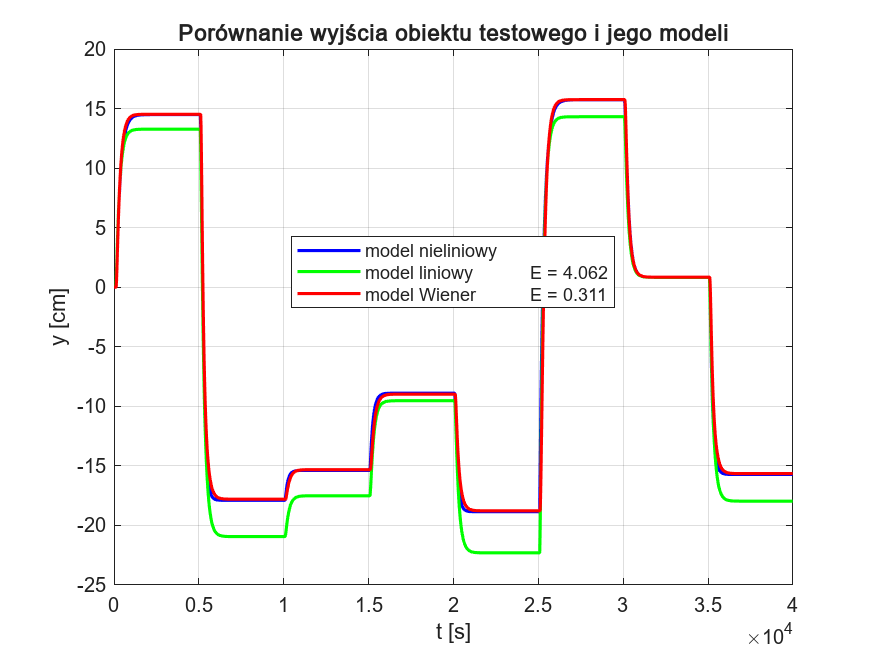
\includegraphics[width=0.7\textwidth]{pictures/WienerNonlinearModel_1}}
\caption{Porównanie modelu Wienera z następnikami liniowymi i nieliniowymi - pierwsza sekwencja.}
\label{first_wien}
\end{figure}

\begin{figure}[p]
\centering
\subfloat[Następniki liniowe]{
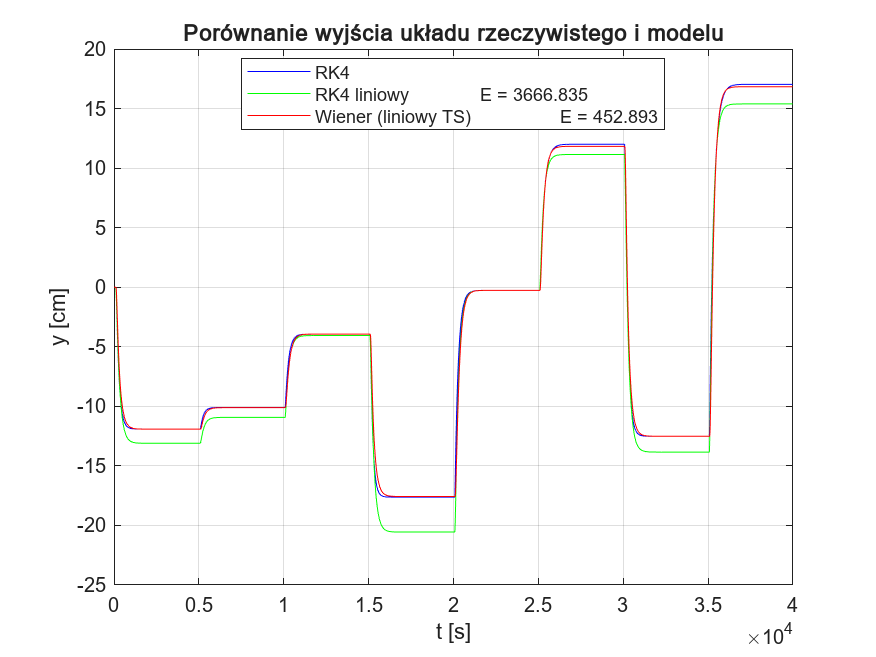
\includegraphics[width=0.75\textwidth]{pictures/WienerLinearModel_2}}
\vspace{0.5cm}
\subfloat[Następniki nieliniowe]{
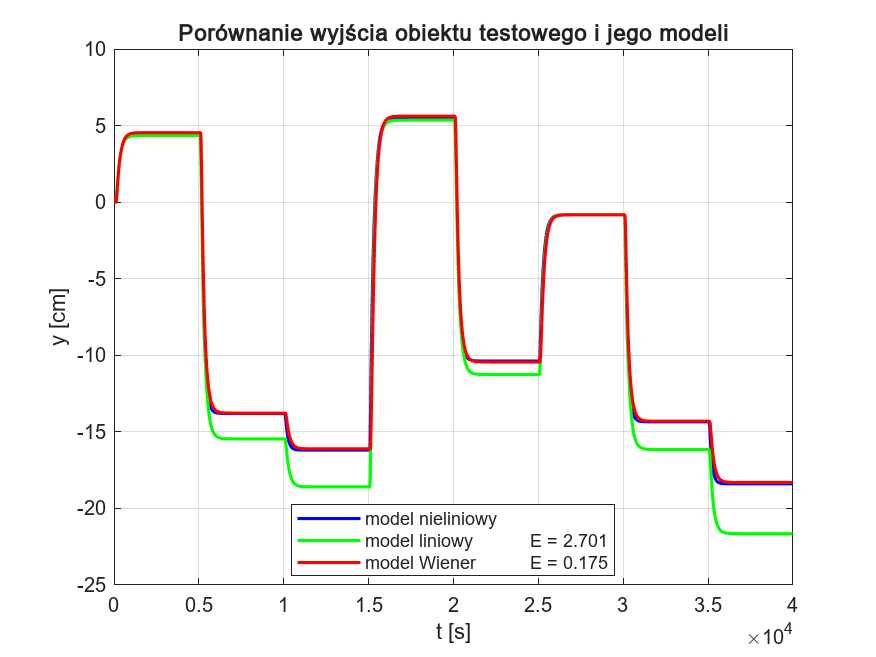
\includegraphics[width=0.75\textwidth]{pictures/WienerNonlinearModel_2}}
\caption{Porównanie modelu Wienera z następnikami liniowymi i nieliniowymi - druga sekwencja.}
\end{figure}

\begin{figure}[p]
\centering
\subfloat[Następniki liniowe]{
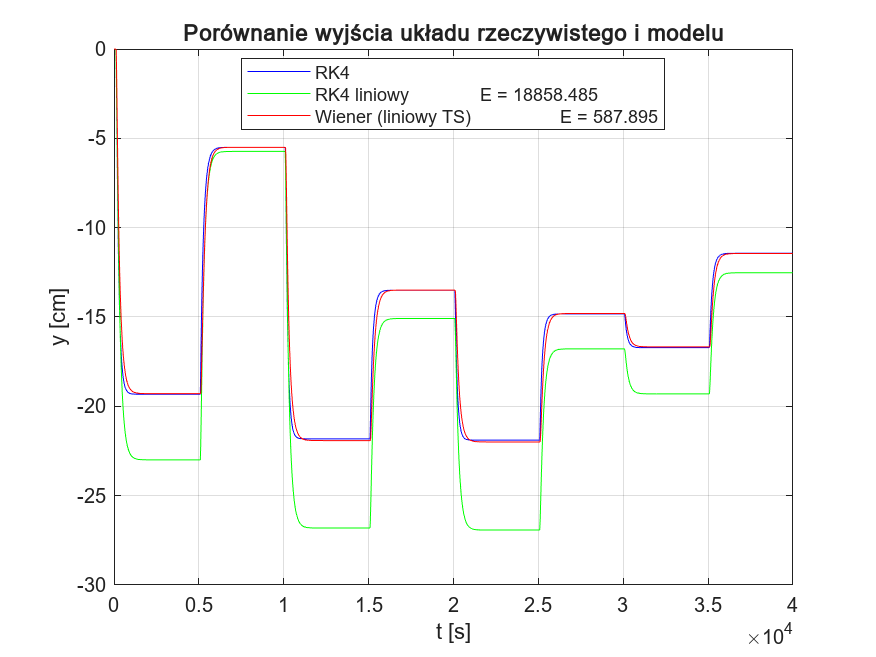
\includegraphics[width=0.75\textwidth]{pictures/WienerLinearModel_3}}
\vspace{0.5cm}
\subfloat[Następniki nieliniowe]{
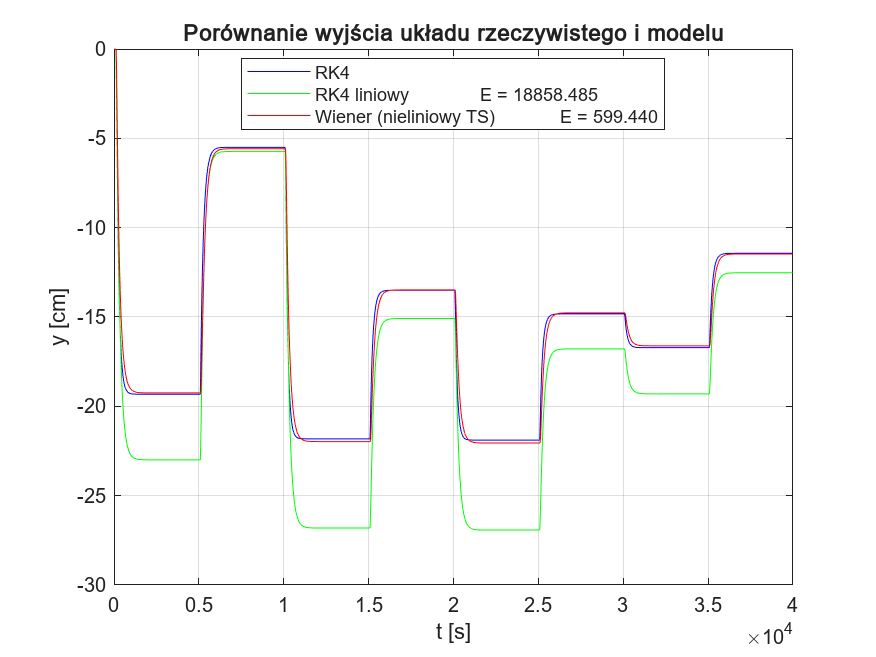
\includegraphics[width=0.75\textwidth]{pictures/WienerNonlinearModel_3}}
\caption{Porównanie modelu Wienera z następnikami liniowymi i nieliniowymi - trzecia sekwencja.}
\end{figure}

\begin{figure}[p]
\centering
\subfloat[Następniki liniowe]{
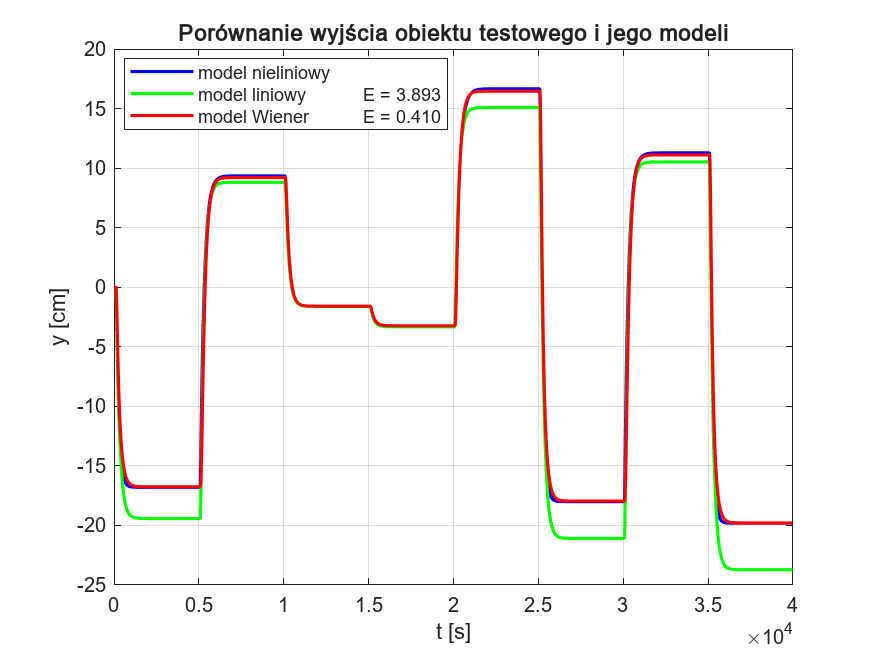
\includegraphics[width=0.75\textwidth]{pictures/WienerLinearModel_4}}
\vspace{0.5cm}
\subfloat[Następniki nieliniowe]{
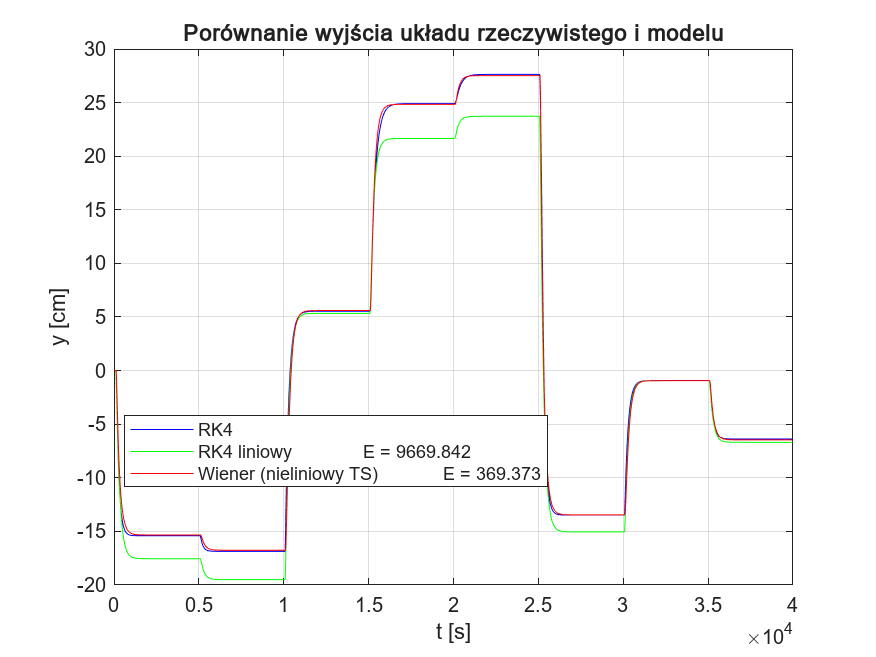
\includegraphics[width=0.75\textwidth]{pictures/WienerNonlinearModel_4}}
\caption{Porównanie modelu Wienera z następnikami liniowymi i nieliniowymi - czwarta sekwencja.}
\end{figure}

\begin{figure}[p]
\centering
\subfloat[Następniki liniowe]{
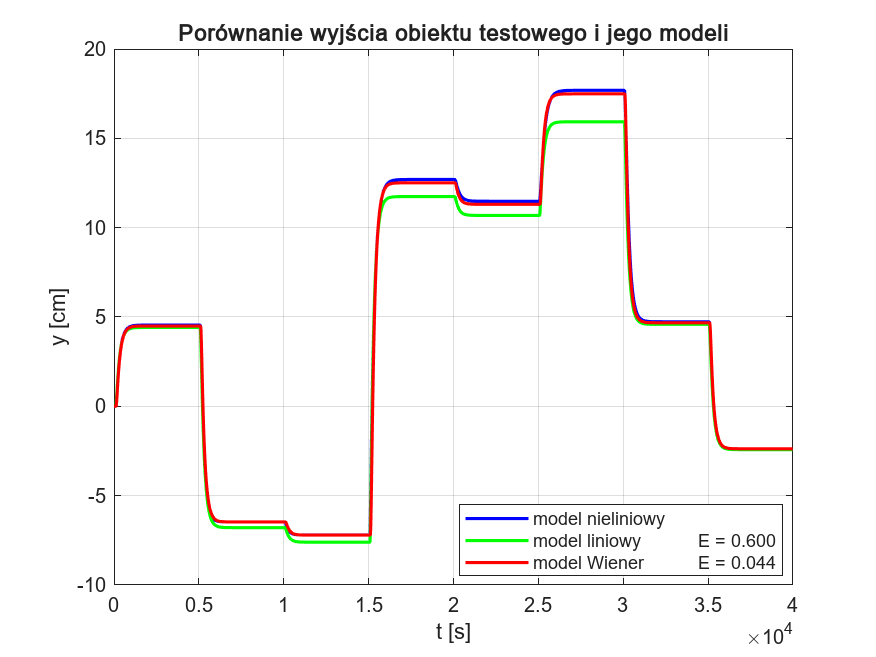
\includegraphics[width=0.75\textwidth]{pictures/WienerLinearModel_5}}
\vspace{0.5cm}
\subfloat[Następniki nieliniowe]{
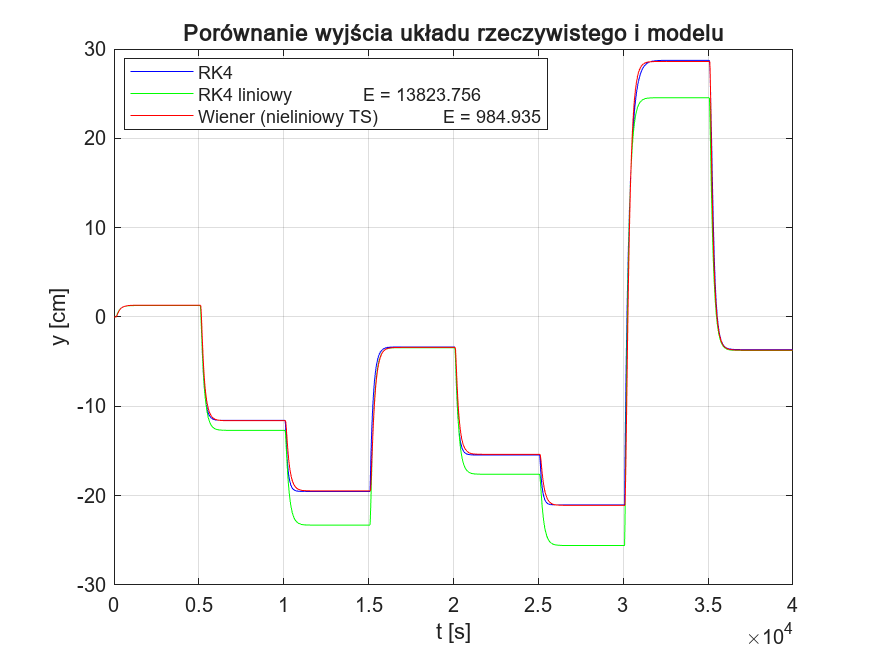
\includegraphics[width=0.75\textwidth]{pictures/WienerNonlinearModel_5}}
\caption{Porównanie modelu Wienera z następnikami liniowymi i nieliniowymi - piąta sekw encja.}
\label{last_wien}
\end{figure}

\newpage

Wyniki zebrane w tab. \ref{comparison_wien} dla modelu Wienera z następnikami liniowymi i nieliniowymi są niemalże identyczne, a ewentualne różnice są pomijalne. Porównując otrzymane rezultaty z tymi otrzymanymi w przypadku modelu Hammersteina okazuje się, że model Wienera jest nieco lepszy, co może wskazywać na większe nieliniowości na wyjściu procesu.
 
\begin{table}[h!]
\centering
\renewcommand{\arraystretch}{1.2}
\begin{tabular}{|>{\centering\arraybackslash}m{2cm}|>{\centering\arraybackslash}m{3cm}|>{\centering\arraybackslash}m{3cm}|>{\centering\arraybackslash}m{3cm}|}
\hline
\multirow{2}{*}{Nr sekwencji} & \multirow{2}{*}{Model liniowy} & \multicolumn{2}{c|}{Model Wienera} \\ \cline{3-4}
 &  & Następniki liniowe & Następniki nieliniowe \\ \hline
1. & $\num{4.062}$ & $\num{0.314}$ & $\num{0.311}$ \\ \hline
2. & $\num{2.701}$ & $\num{0.173}$ & $\num{0.175}$ \\ \hline
3. & $\num{1.283}$ & $\num{0.163}$ & $\num{0.157}$ \\ \hline
4. & $\num{3.893}$ & $\num{0.410}$ & $\num{0.409}$ \\ \hline
5. & $\num{0.600}$ & $\num{0.044}$ & $\num{0.035}$ \\ \hline
\end{tabular}
\caption{Porównanie modeli.}
\label{comparison_wien}
\end{table}

Udało się osiągnąć zamierzony efekt - mniejsza liczba reguł, bez utraty dokładności.
\chapter{Podsumowanie}
W trakcie wykonywania projektu oraz identyfikując dany obiekt regulacji automatycznej nasunęło się kilka wniosków, które postarano się opisać poniżej.

Modele Hammersteina składają się z nieliniowego bloku wejściowego, który jest połączony szeregowo z liniowym dynamicznym blokiem. Nieliniowość jest zazwyczaj statyczna i jest aplikowana do sygnału wejściowego przed jego przetworzeniem przez liniowy system dynamiczny. Ten rodzaj modelu jest używany do opisu systemów, gdzie nieliniowość występuje na wejściu, a reszta systemu zachowuje się liniowo. Modele Hammersteina są użyteczne w identyfikacji systemów i projektowaniu regulatorów.

Modele Wienera, odwrotnie do modeli Hammersteina, mają liniowy dynamiczny blok na wejściu, który jest połączony szeregowo z nieliniowym blokiem wyjściowym. Liniowy blok dynamiczny przetwarza sygnał wejściowy, który następnie przechodzi przez nieliniowy blok. Modele te są stosowane, gdy nieliniowość występuje na wyjściu systemu, po przetworzeniu przez liniowy system dynamiczny. Modele Wienera są przydatne w analizie systemów z nieliniowymi elementami wyjściowymi.

Stosowanie modeli Hammersteina i Wienera w obiektach regulacji automatycznej jest ważne, ponieważ pozwalają one na dokładniejsze modelowanie rzeczywistych systemów, które często zawierają zarówno elementy liniowe, jak i nieliniowe. Dzięki nim można lepiej zrozumieć zachowanie takich systemów i opracować bardziej precyzyjne i skuteczne strategie regulacji. To z kolei prowadzi do poprawy wydajności, stabilności i niezawodności systemów automatyki. Integracja tych modeli w procesie projektowania systemów automatyki umożliwia także lepsze przewidywanie i kompensowanie nieliniowych efektów w działaniu systemów.

Jak można było zauważyć na zaprezentowanych wykresach, zaimplementowanie nieliniowej statyki, którą poprzedzała, bądź występowała po niej, liniowa dynamika diametralnie poprawiała jakość opisu obiektu. W każdym z rozpatrywanych przypadków udało się osiągnąć założone kryterium jakości, którym był błąd średnio kwadratowy, nie większy niż $\num{0.1}$. 

%\begin{table}[h!]
%\centering
%\begin{tabular}{>{\centering\arraybackslash}p{3cm}|>{\centering\arraybackslash}p{3cm}|>{\centering\arraybackslash}p{3cm}|>{\centering\arraybackslash}p{3cm}|>{\centering\arraybackslash}p{3cm}}
% & \multicolumn{2}{>{\centering\arraybackslash}p{6cm}|}{Model dynamiczny} &  \multicolumn{2}{>{\centering\arraybackslash}p{6cm}}{Model Wienera} \\ \hline
% & ARX & OE & ARX & OE \\ \hline
%$I$ sekwencja & & & & \\
%$II$ sekwencja & & & & \\
%$III$ sekwencja & & & & 
%\end{tabular}
%\caption{Błędy zbioru uczącego.}
%\end{table}
%
%\begin{table}[h!]
%\centering
%\begin{tabular}{>{\centering\arraybackslash}p{3cm}|>{\centering\arraybackslash}p{3cm}|>{\centering\arraybackslash}p{3cm}|>{\centering\arraybackslash}p{3cm}|>{\centering\arraybackslash}p{3cm}}
% & \multicolumn{2}{>{\centering\arraybackslash}p{6cm}|}{Model dynamiczny} &  \multicolumn{2}{>{\centering\arraybackslash}p{6cm}}{Model Wienera} \\ \hline
% & ARX & OE & ARX & OE \\ \hline
%$I$ sekwencja & & & & \\
%$II$ sekwencja & & & & \\
%$III$ sekwencja & & & & 
%\end{tabular}
%\caption{Błędy zbioru weryfikującego.}
%\end{table}

\listoffigures
%\listoftables
\end{document}